\pdfminorversion=7%
\documentclass[aspectratio=169,mathserif,notheorems]{beamer}%
%
\xdef\bookbaseDir{../../bookbase}%
\xdef\sharedDir{../../shared}%
\RequirePackage{\bookbaseDir/styles/slides}%
\RequirePackage{\sharedDir/styles/styles}%
%
%
\subtitle{Getting Started}%
%
\begin{document}%
\startPresentation%
%
\section{Introduction}%
%
\begin{frame}%
\frametitle{Introduction}%
\begin{itemize}%
\item This will be a practical course, so we should get started with practical things right away.%
\item<2-> In order to do practical things, we need to have all the necessary software on our computer.%
\item<3-> Here we discuss what software you need and how you can install it.%
\item<4-> We will also discuss how to write a simple program in a \python\ editor and how we can run \python\ programs.%
\item<5-> Indeed, we provide a big load of example programs in this course, based on which we will discuss the different aspects of \python\ programming.%
\item<6-> So, finally, we will also check how you can download these example programs.%
\end{itemize}%
\end{frame}%
%
\begin{frame}%
\frametitle{Software Needed for \python\ Software Development}%
\begin{itemize}%
\item What software is necessary to do \python\ programming?\uncover<2->{ \python.\uncover<3->{ We will discuss how to install \python.}}%
\item<4-> With the programming language \python\ alone, you cannot really do much \emph{conveniently}.%
\item<5-> You need a nice editor in which you can write the programs\uncover<6->{, where you can also directly execute and test your programs\uncover<7->{, where you can work with a work with a version control system like \git\cite{S2023LG,T2024BGAGVCPMATFTND}.}}%
\item<8-> Such  called an Integrated Development Environment~(IDE).\uncover<9->{We will use the \pycharm\ IDE\cite{VHN2023HOADWP,Y2022PPADT}.\uncover<10->{ Se we will discuss how you can install it.}}%
\item<11-> As operating system, I strongly recommend using \linux\cite{T1999TLE,B2022ELATCL,H2022LML} for programming, work, and research.\uncover<12->{ I am using \ubuntu\ \linux\cite{CN2020ULB}.}%
%
\item<13-> I will provide examples and instructions for both \ubuntu\ and \microsoftWindows\cite{B2023W1IO}.%
\end{itemize}%
\end{frame}%
%
\section{Installing \python}%
%
\begin{frame}%
\frametitle{Installing \python}%
\begin{itemize}%
\item There are two major versions of \python: \python~2 and \python~3.%
\item<2-> \alert{We focus entirely on \python~3.}%
\item<3-> We assume that you have installed \pythonWithVersion\ or newer.
\item<4-> We here provide some brief setup instructions.
\item<5->More help can be found at the following resources\uncover<6->{:%
%
\begin{enumerate}%
\item the official \python\ setup and usage page~\url{https://docs.python.org/3/using}\cite{PSF:P3D:PSAU},%
\item the \python\ Downloads at~\url{https://www.python.org/downloads}, and%
\item the \python~3 Installation \& Setup Guide at~\url{https://realpython.com/installing-python}%
\end{enumerate}}%
\end{itemize}%
\end{frame}%
%
\begin{frame}[fragile,t]
\frametitle{Installing \python\ under \ubuntu\ \linux}%
\begin{itemize}%
\item Under \ubuntu\ \linux, \python\ will usually installed by default.%
\end{itemize}%
\locate{2}{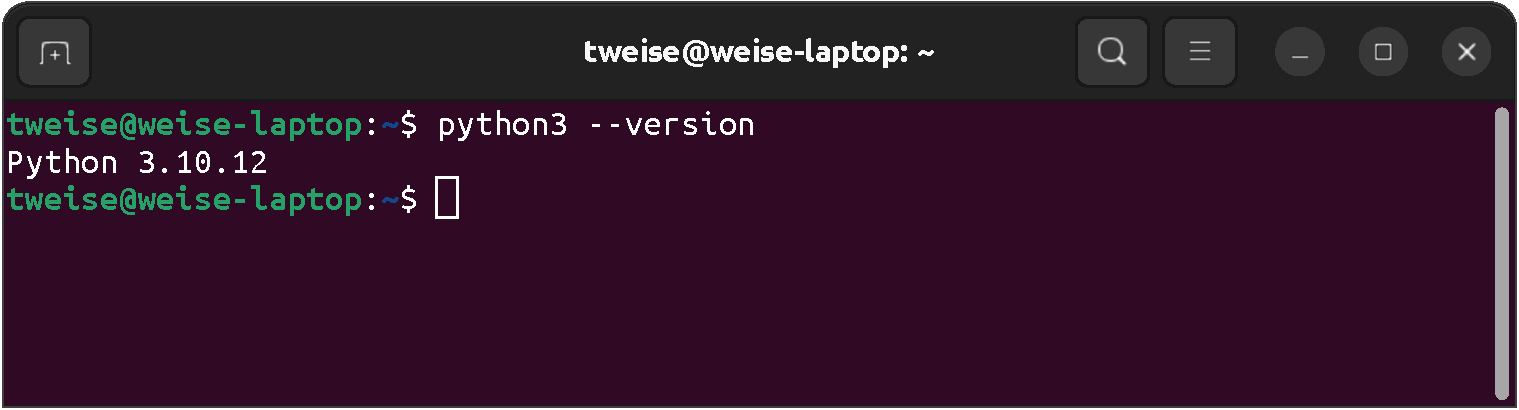
\includegraphics[width=0.65\paperwidth]{graphics/pythonUnderUbuntu/ubuntuTerminalPythonVersion}}{0.05}{0.35}%
\locate{2}{\parbox{0.2\paperwidth}{to open a \linux\ terminal, press \ubuntuTerminal}}{0.73}{0.4}%
\end{frame}
%
\begin{frame}[fragile,t]
\frametitle{Installing \python\ under \microsoftWindows}%
\uncover<-1>{%
\begin{itemize}%
\item Under \microsoftWindows, \python\ might not be installed by default.%
\end{itemize}}%
%
\locate{2}{\tightbox{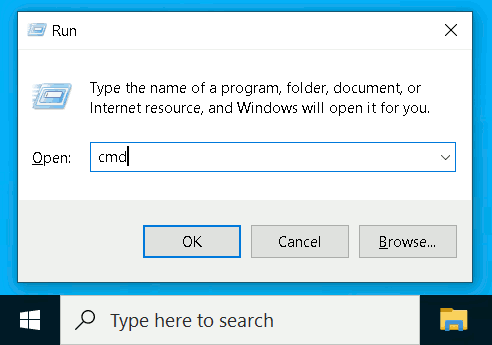
\includegraphics[width=0.65\paperwidth]{graphics/installingPythonWindows/installingPythonWindows01openTerminal}}}{0.05}{0.15}%
\locate{2}{\parbox{0.2\paperwidth}{to open a \microsoftWindows\ terminal, \windowsTerminal}}{0.73}{0.3}%
\locate{3}{\tightbox{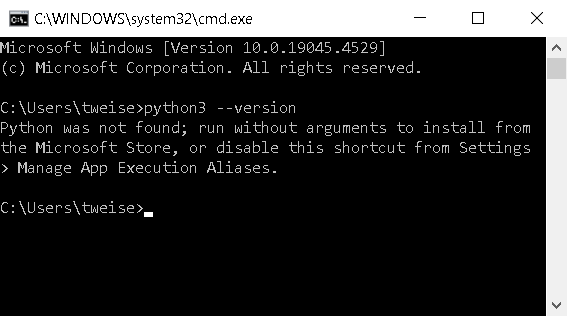
\includegraphics[width=0.7\paperwidth]{graphics/installingPythonWindows/installingPythonWindows02pythonVersion}}}{0.15}{0.15}%
\locate{4}{\tightbox{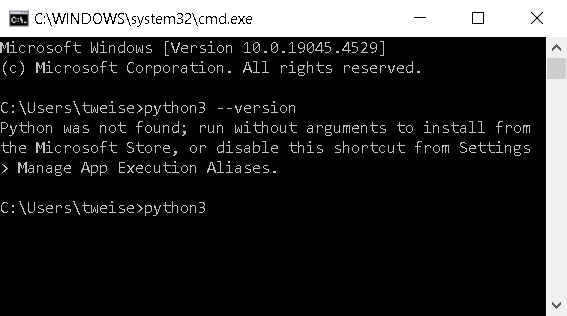
\includegraphics[width=0.7\paperwidth]{graphics/installingPythonWindows/installingPythonWindows03python}}}{0.15}{0.15}%
\locate{5}{\tightbox{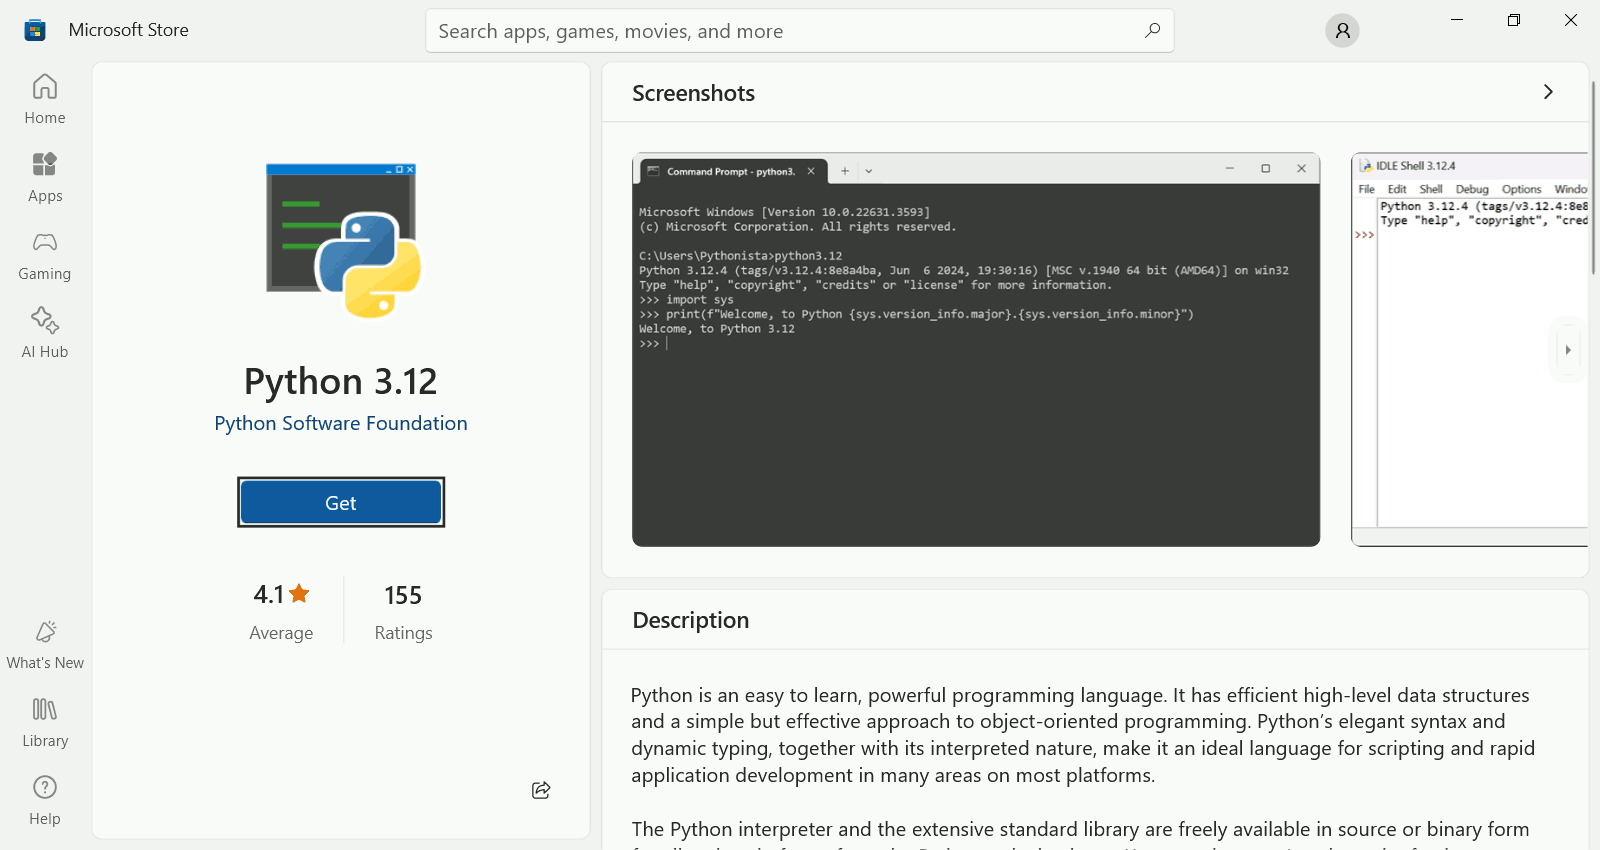
\includegraphics[width=0.8\paperwidth]{graphics/installingPythonWindows/installingPythonWindows04installGet}}}{0.1}{0.15}%
\locate{6}{\tightbox{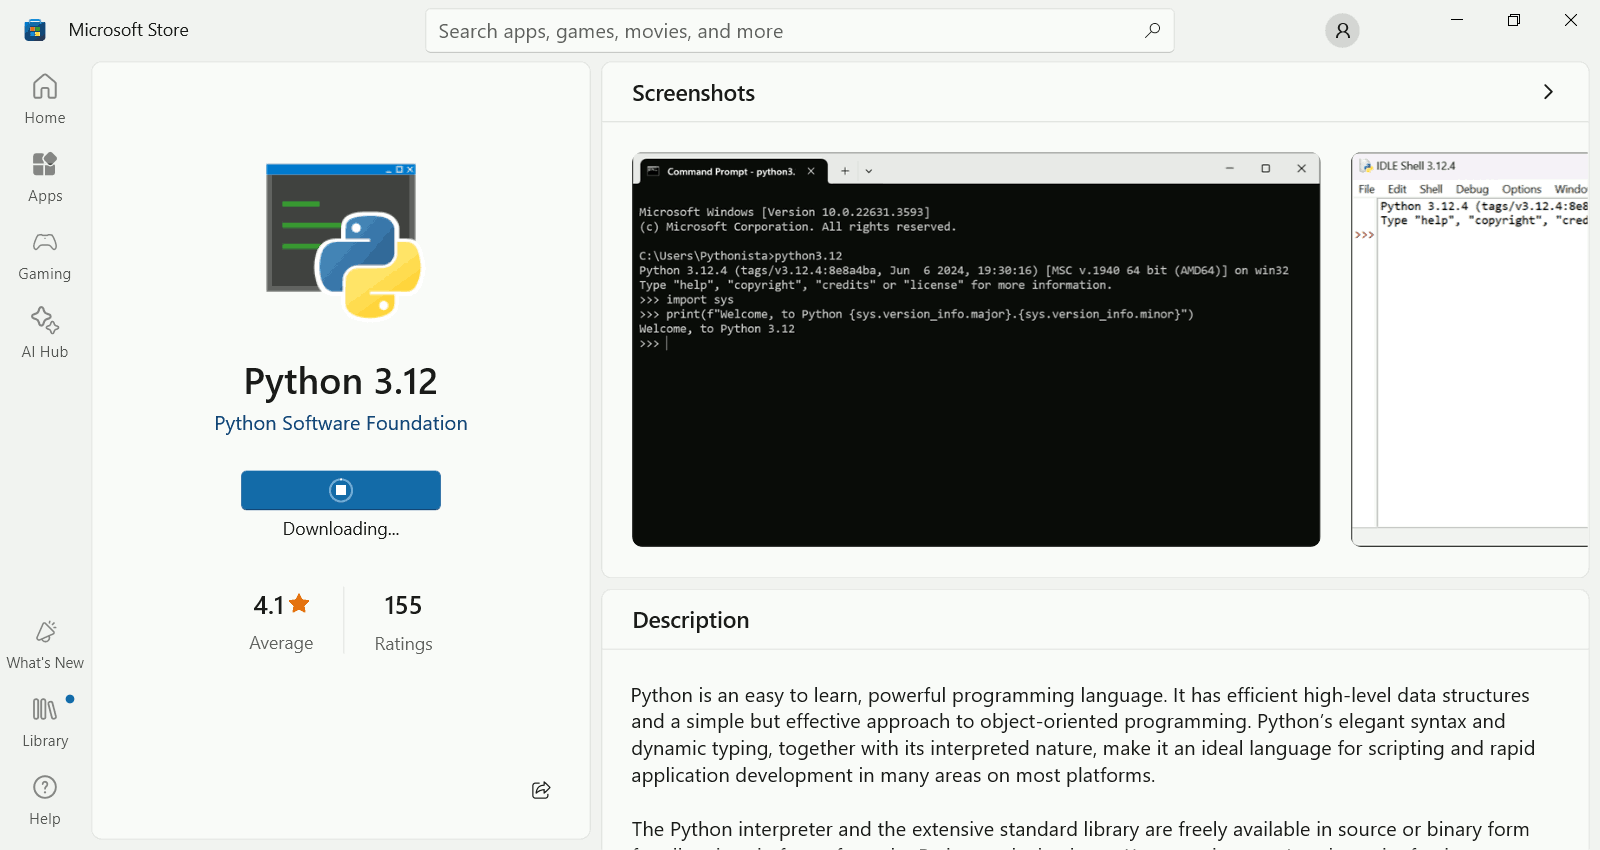
\includegraphics[width=0.8\paperwidth]{graphics/installingPythonWindows/installingPythonWindows05downloading}}}{0.1}{0.15}%
\locate{7}{\tightbox{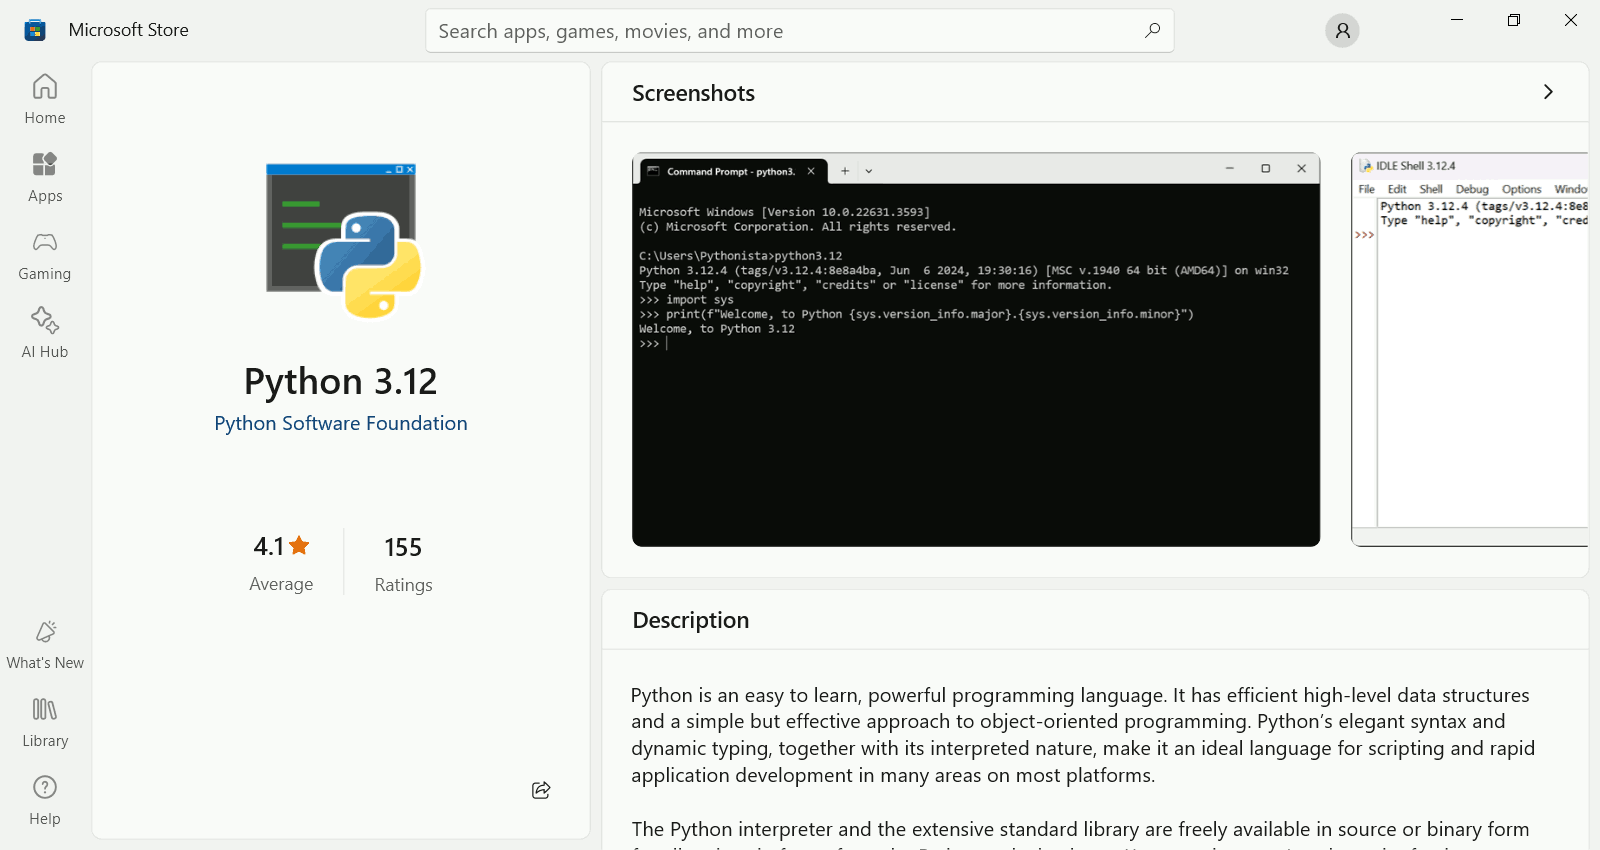
\includegraphics[width=0.8\paperwidth]{graphics/installingPythonWindows/installingPythonWindows06finished}}}{0.1}{0.15}%
\locate{8}{\tightbox{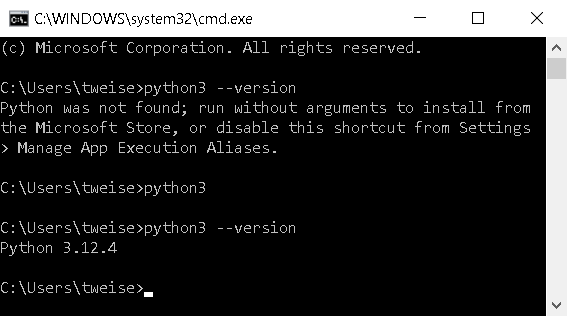
\includegraphics[width=0.7\paperwidth]{graphics/installingPythonWindows/installingPythonWindows07pythonVersion}}}{0.15}{0.15}%
\end{frame}
%
\section{Installing \pycharm}%
%
\begin{frame}%
\frametitle{Installing \pycharm}%
\begin{itemize}%
\item We now install a nice IDE for \python\ software development:~\pycharm.%
\item<2-> Its community edition is freely available.%
\item<3-> The installation guide for \pycharm\ can be found at \url{https://www.jetbrains.com/help/pycharm/installation-guide.html}.%
\end{itemize}%
\end{frame}%
%
\begin{frame}[fragile,t]
\frametitle{Installing \pycharm\ under \ubuntu\ \linux}%
\begin{itemize}%
\item Under \ubuntu\ \linux, \pycharm\ can be installed as snap\cite{C2025SD,J2024PCPCE}.%
\end{itemize}%
\locate{2}{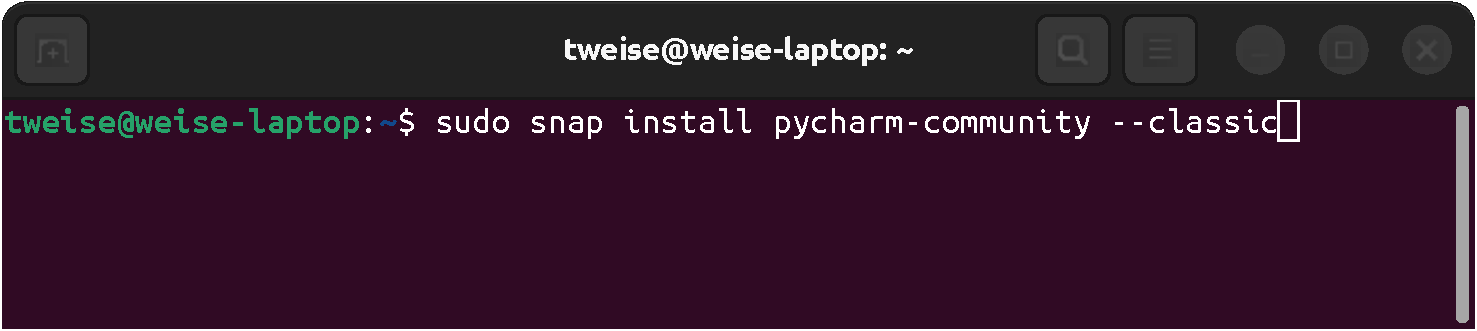
\includegraphics[width=0.65\paperwidth]{graphics/installingPyCharmUbuntu/installingPyCharmUbuntu01snapInstall}}{0.05}{0.35}%
\locate{2}{\parbox{0.2\paperwidth}{to open a \linux\ terminal, press \ubuntuTerminal}}{0.73}{0.4}%
\locate{3}{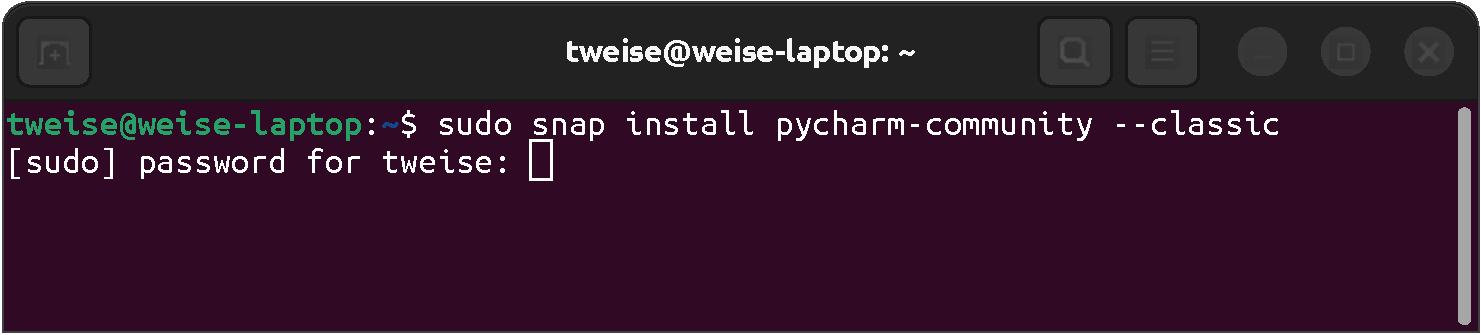
\includegraphics[width=0.75\paperwidth]{graphics/installingPyCharmUbuntu/installingPyCharmUbuntu02sudo}}{0.125}{0.35}%
\locate{4}{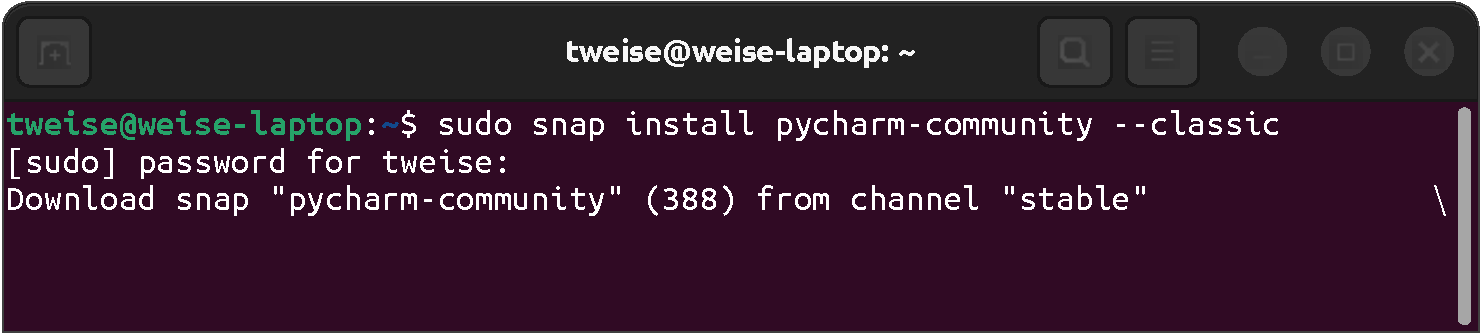
\includegraphics[width=0.75\paperwidth]{graphics/installingPyCharmUbuntu/installingPyCharmUbuntu03snapInstall}}{0.125}{0.35}%
\locate{5}{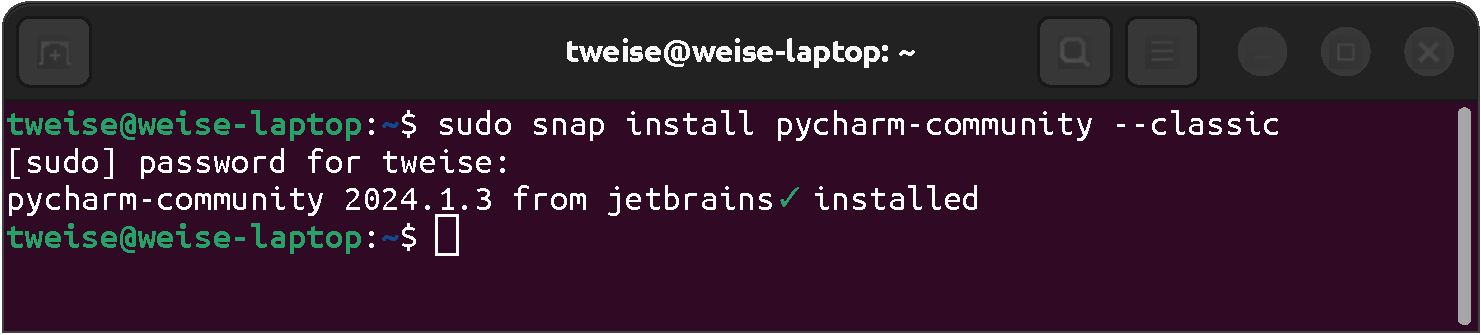
\includegraphics[width=0.75\paperwidth]{graphics/installingPyCharmUbuntu/installingPyCharmUbuntu05snapInstallFinished}}{0.125}{0.35}%
\locate{6}{\tightbox{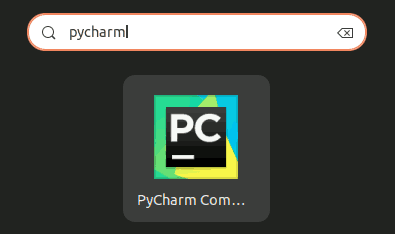
\includegraphics[width=0.55\paperwidth]{graphics/installingPyCharmUbuntu/installingPyCharmUbuntu06launcher}}}{0.125}{0.35}%
\locate{6}{\parbox{0.2\paperwidth}{Open the launcher by pressing \OSwin\ and type in \bashil{pycharm}}}{0.73}{0.3}%%
\locate{7}{\tightbox{
\includegraphics[width=0.5\paperwidth]{graphics/installingPyCharmUbuntu/installingPyCharmUbuntu07welcome}}}{0.25}{0.25}%
\locate{8}{\tightbox{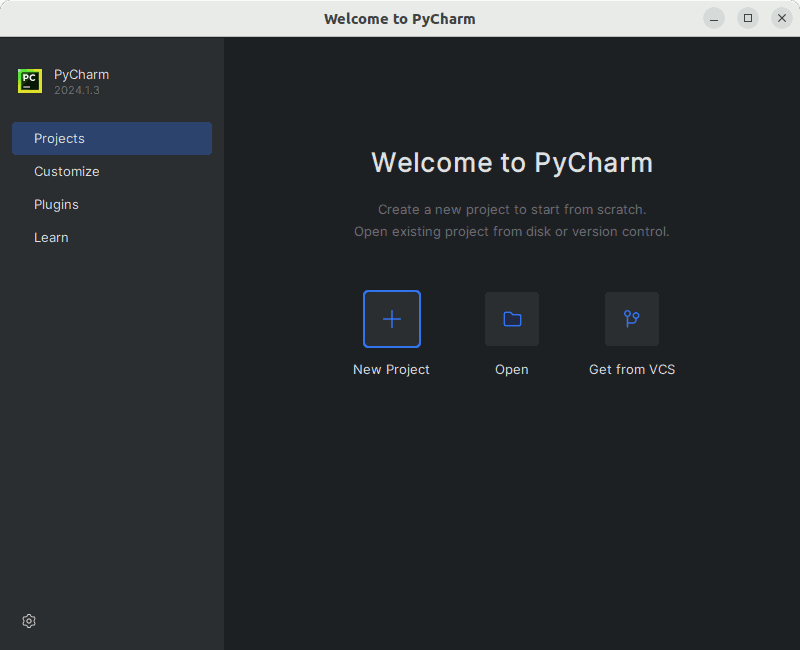
\includegraphics[width=0.5\paperwidth]{graphics/installingPyCharmUbuntu/installingPyCharmUbuntu08pycharm}}}{0.25}{0.23}%
%
\end{frame}
%
\begin{frame}[fragile,t]
\frametitle{Installing \pycharm\ under \ubuntu\ \linux}%
\begin{itemize}%
\item Under \microsoftWindows, you need to download and install the \pycharm\ Community Edition installation executable from \url{https://www.jetbrains.com/pycharm/download}.%
\end{itemize}%
%
\locate{2}{\tightbox{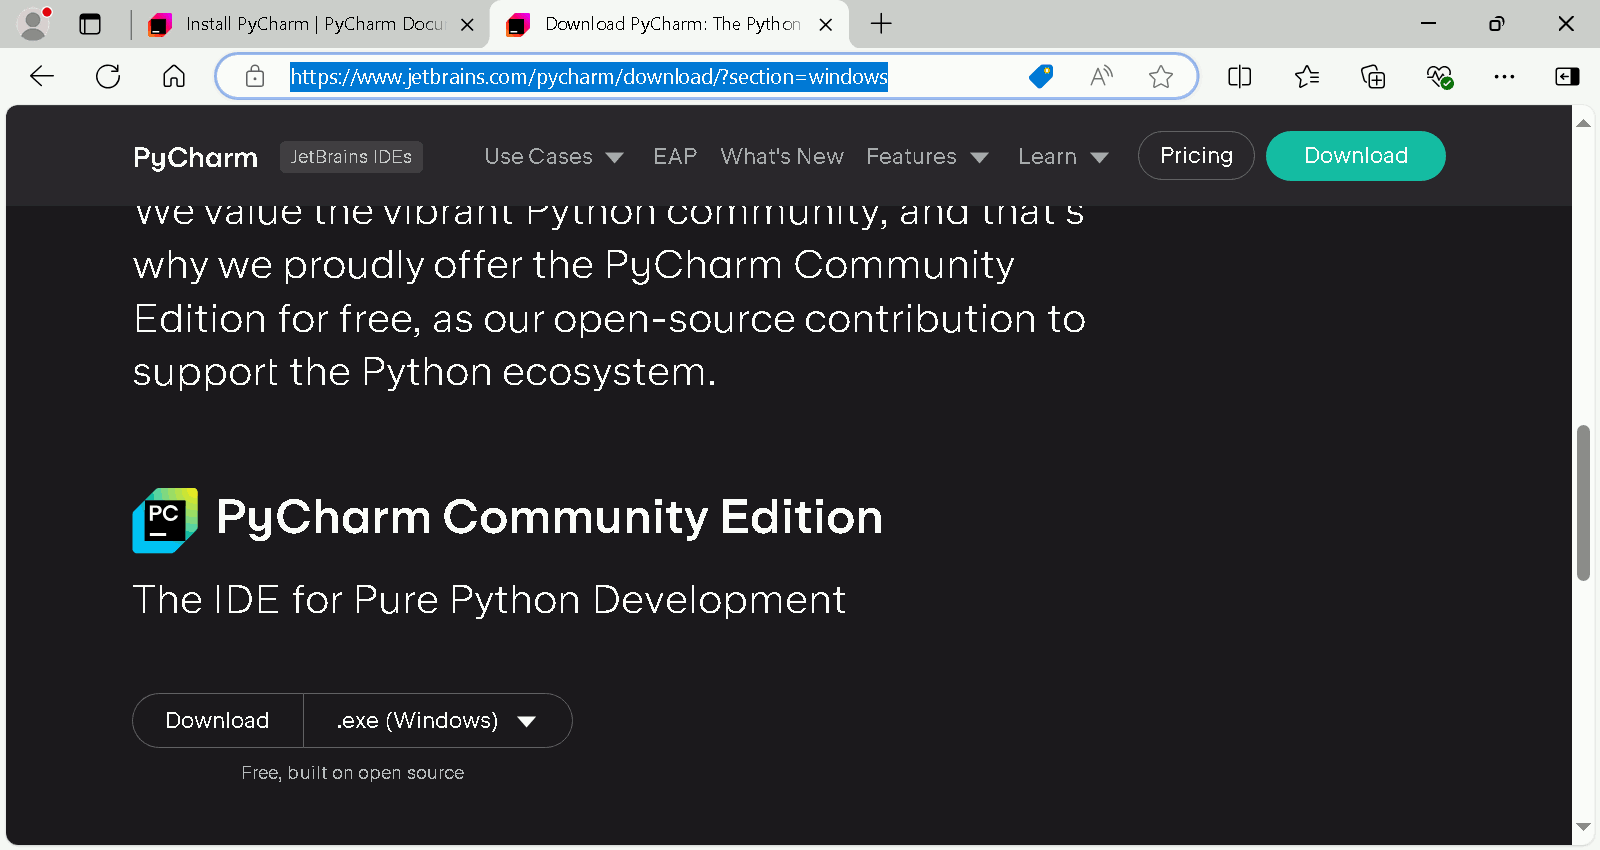
\includegraphics[width=0.7\paperwidth]{graphics/installingPyCharmWindows/installingPyCharmWindows01download}}}{0.15}{0.29}%
\locate{3}{\tightbox{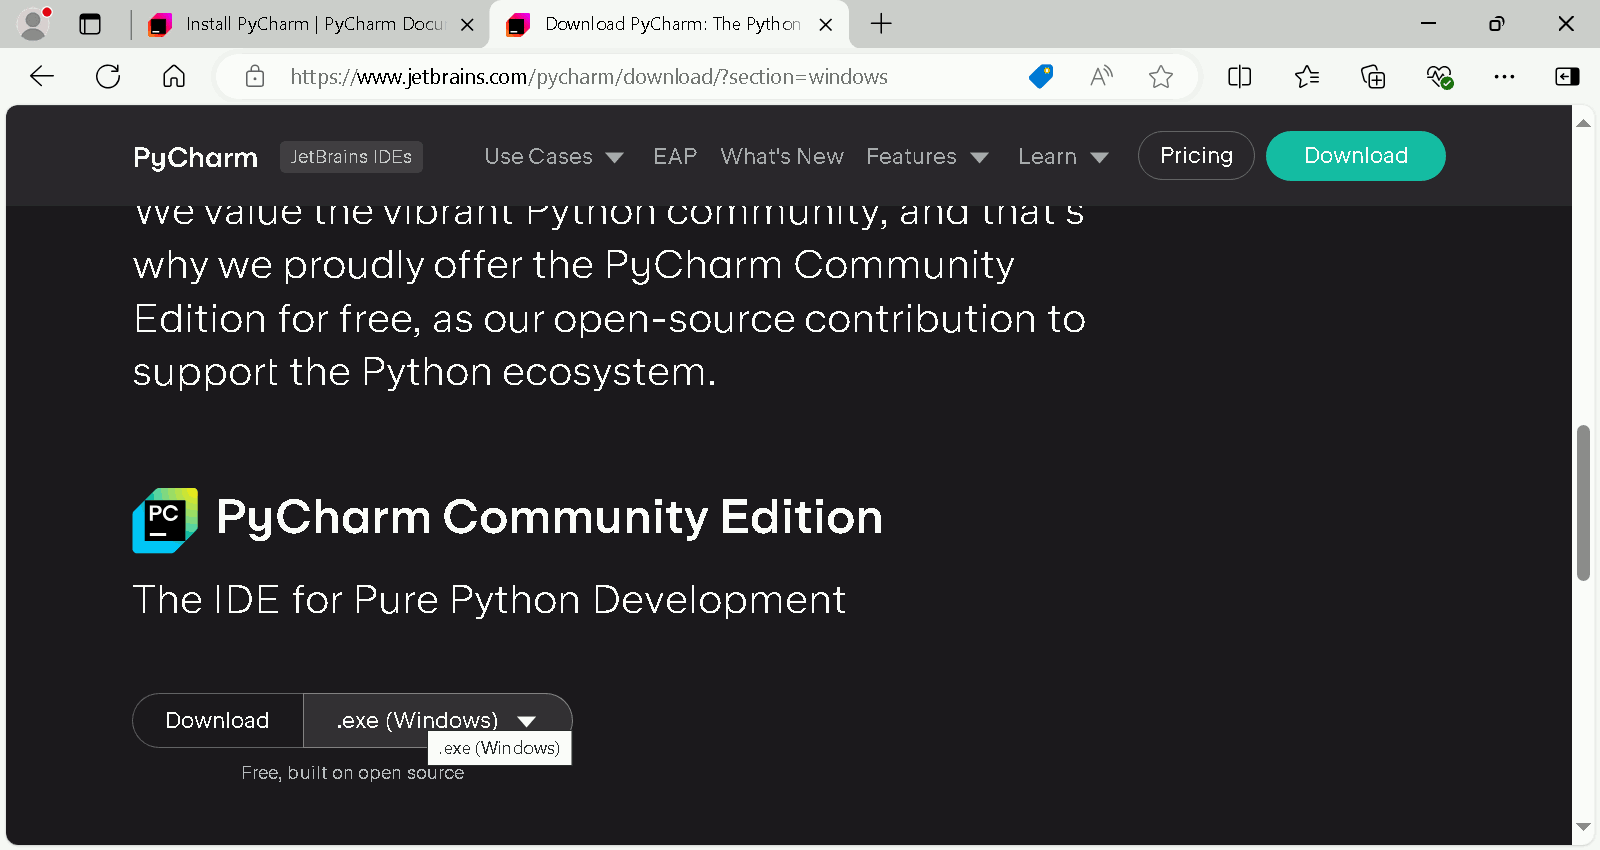
\includegraphics[width=0.7\paperwidth]{graphics/installingPyCharmWindows/installingPyCharmWindows02download}}}{0.15}{0.29}%
\locate{4}{\tightbox{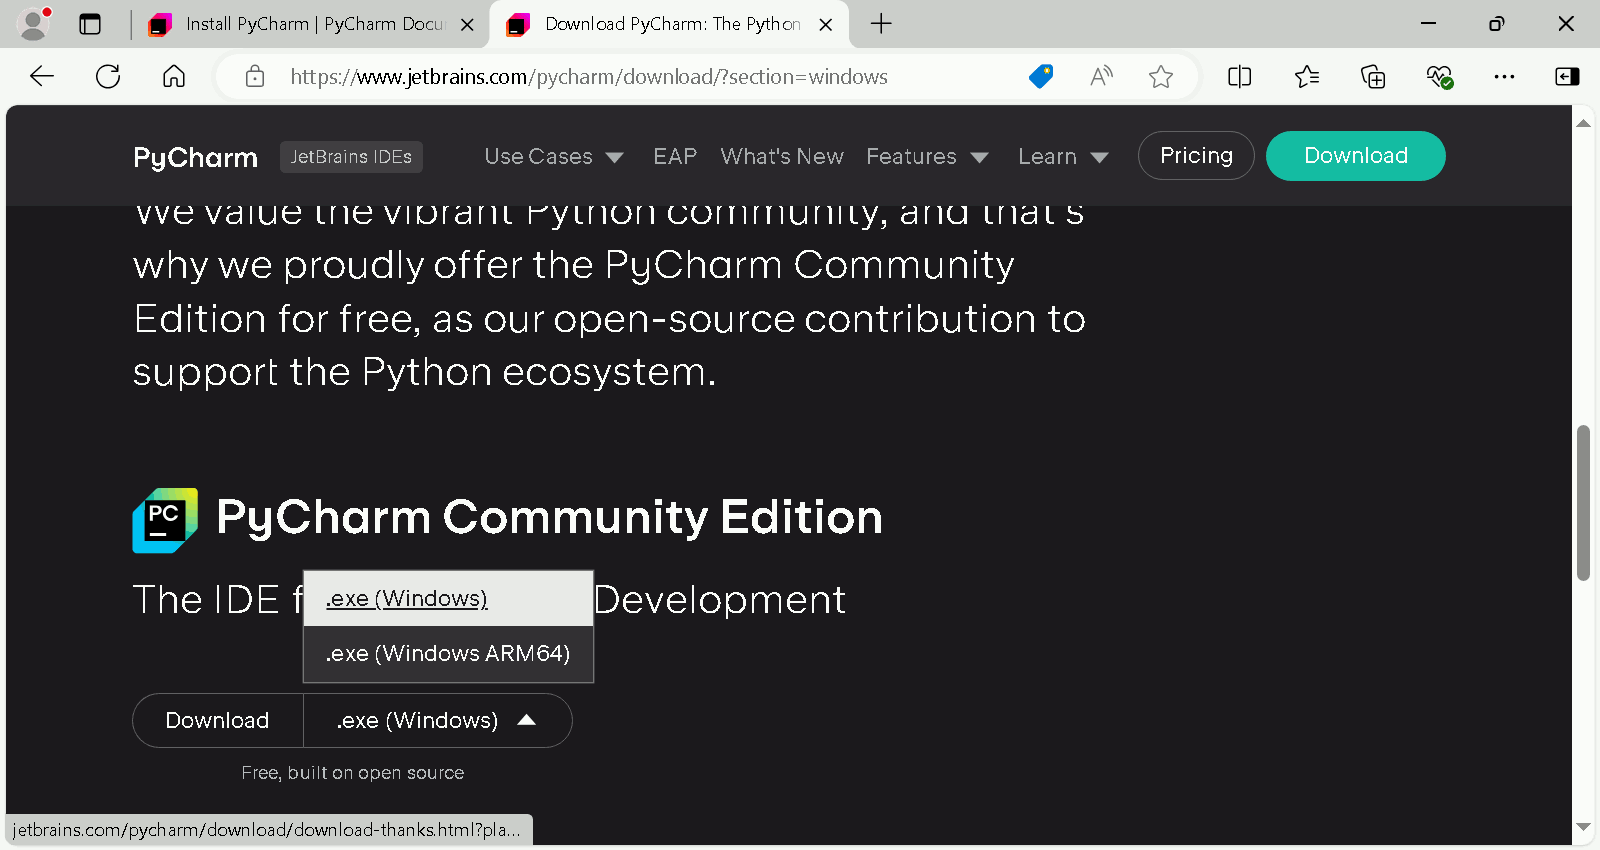
\includegraphics[width=0.7\paperwidth]{graphics/installingPyCharmWindows/installingPyCharmWindows03download}}}{0.15}{0.29}%
\locate{5}{\tightbox{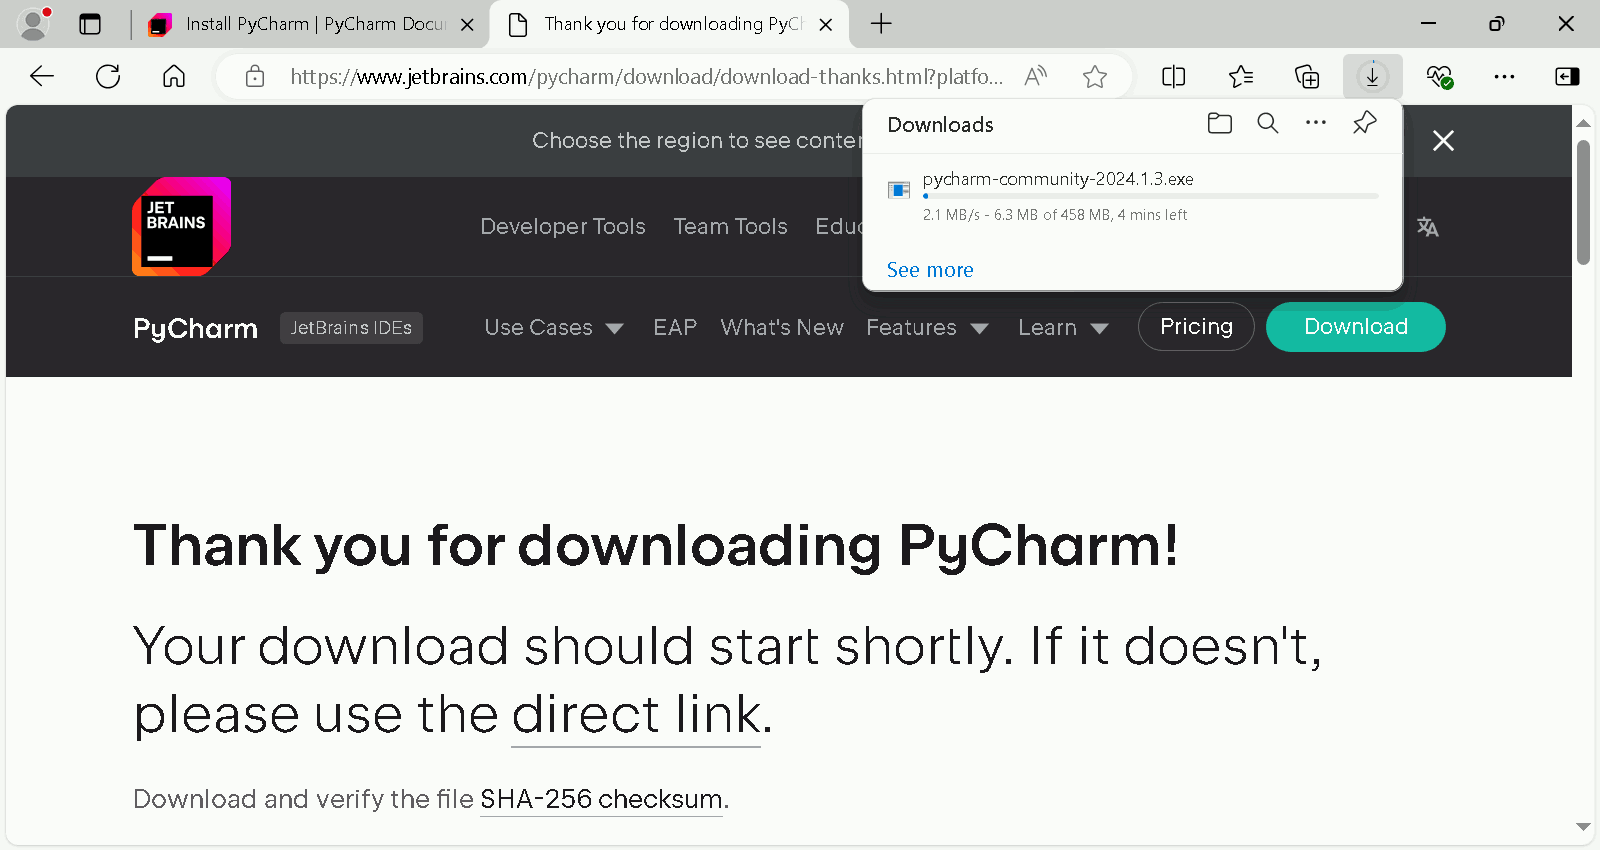
\includegraphics[width=0.7\paperwidth]{graphics/installingPyCharmWindows/installingPyCharmWindows04download}}}{0.15}{0.29}%
\locate{6}{\tightbox{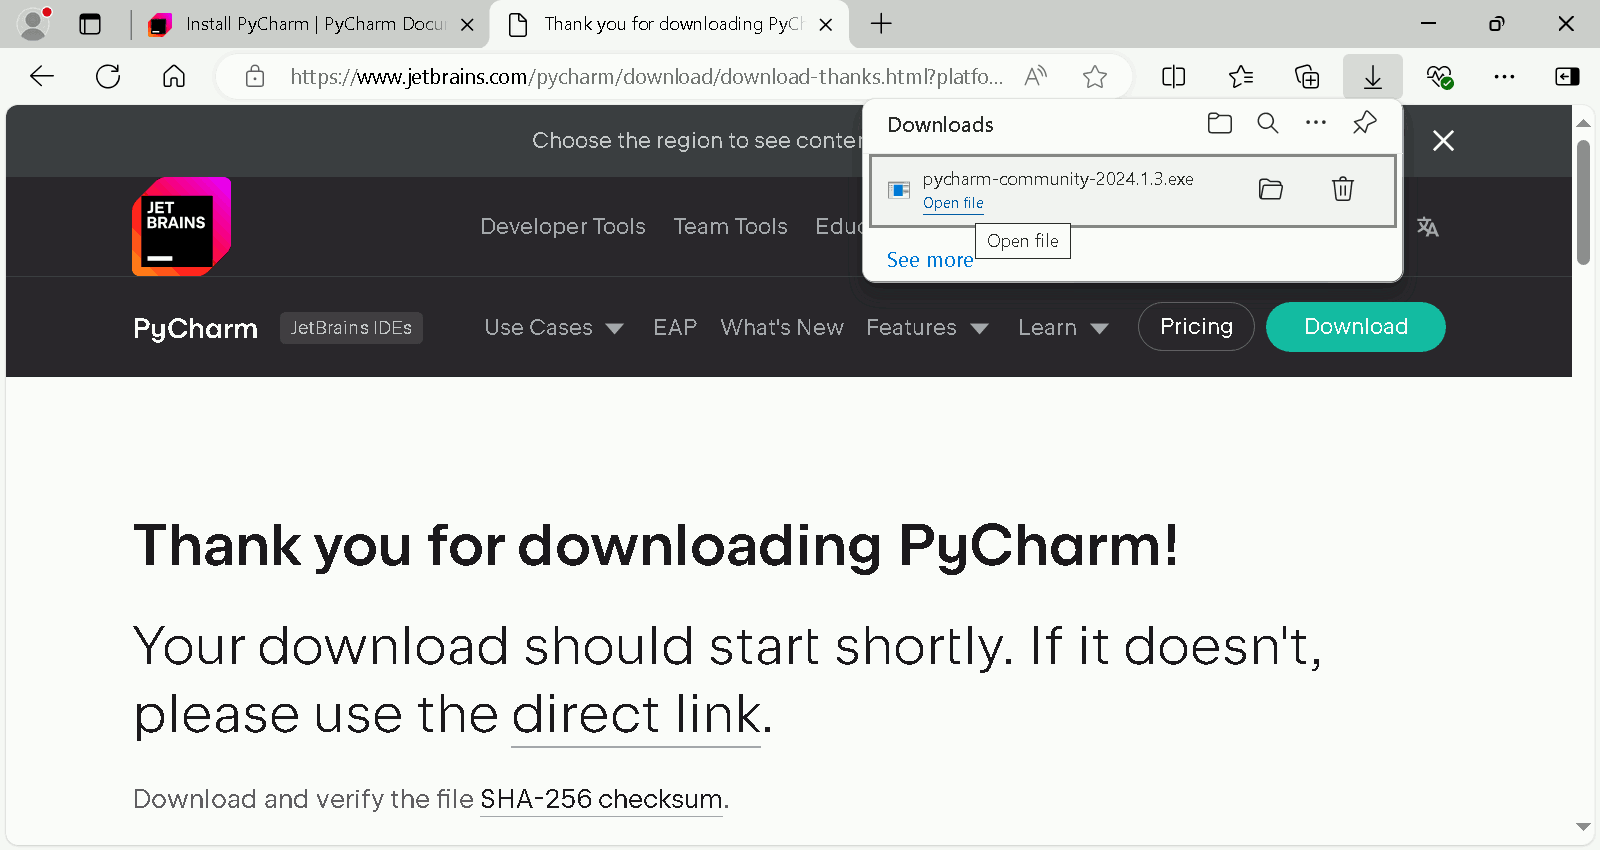
\includegraphics[width=0.7\paperwidth]{graphics/installingPyCharmWindows/installingPyCharmWindows05runInstaller}}}{0.15}{0.29}%
\locate{7}{\tightbox{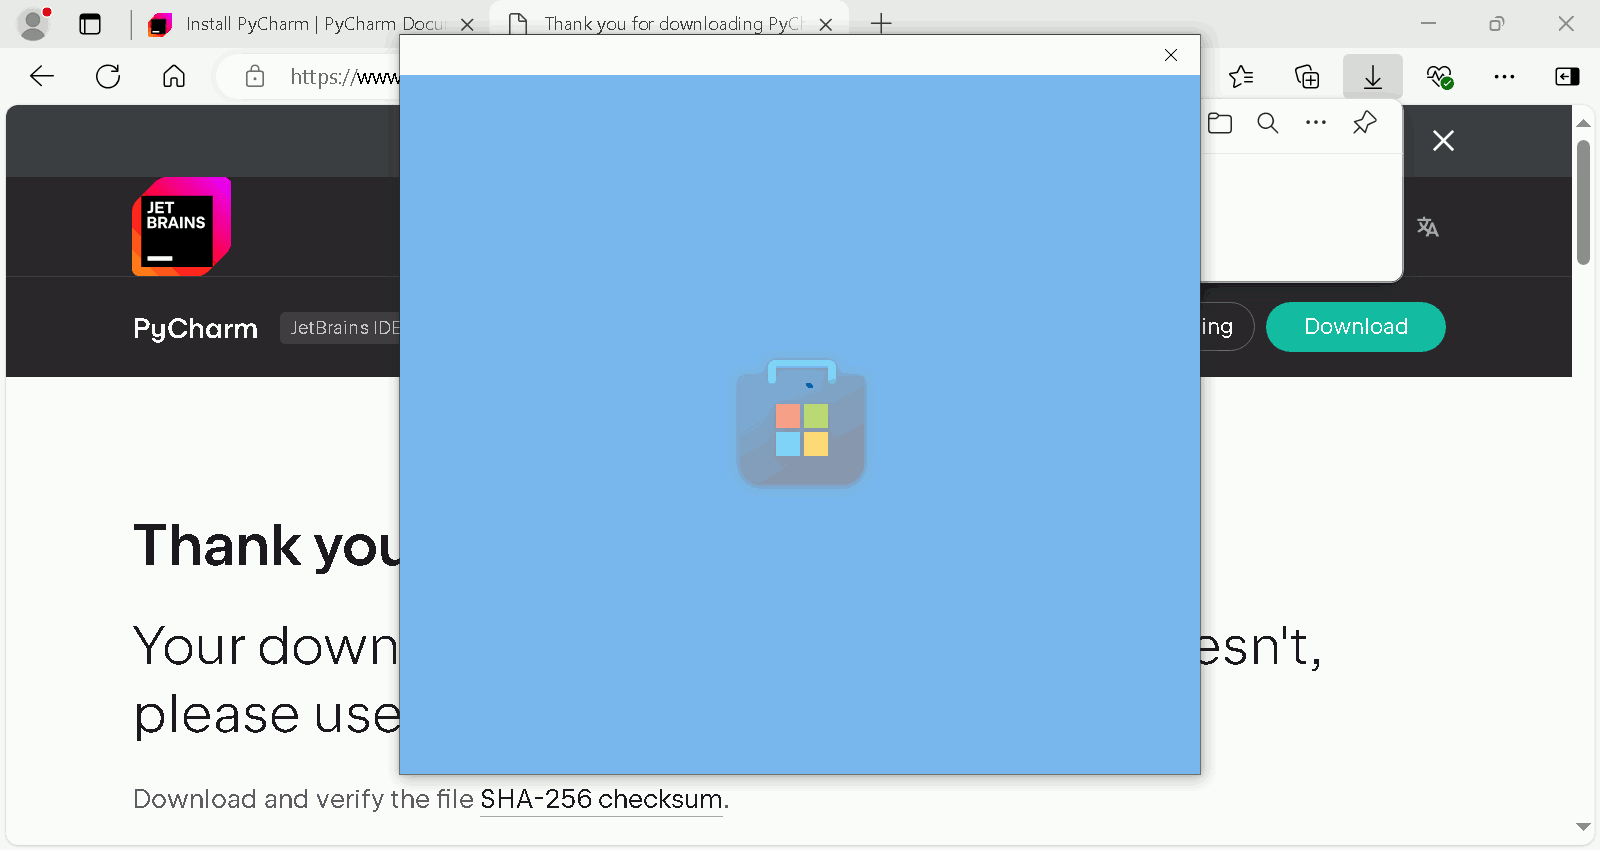
\includegraphics[width=0.7\paperwidth]{graphics/installingPyCharmWindows/installingPyCharmWindows06runInstaller}}}{0.15}{0.29}%
\locate{8}{\tightbox{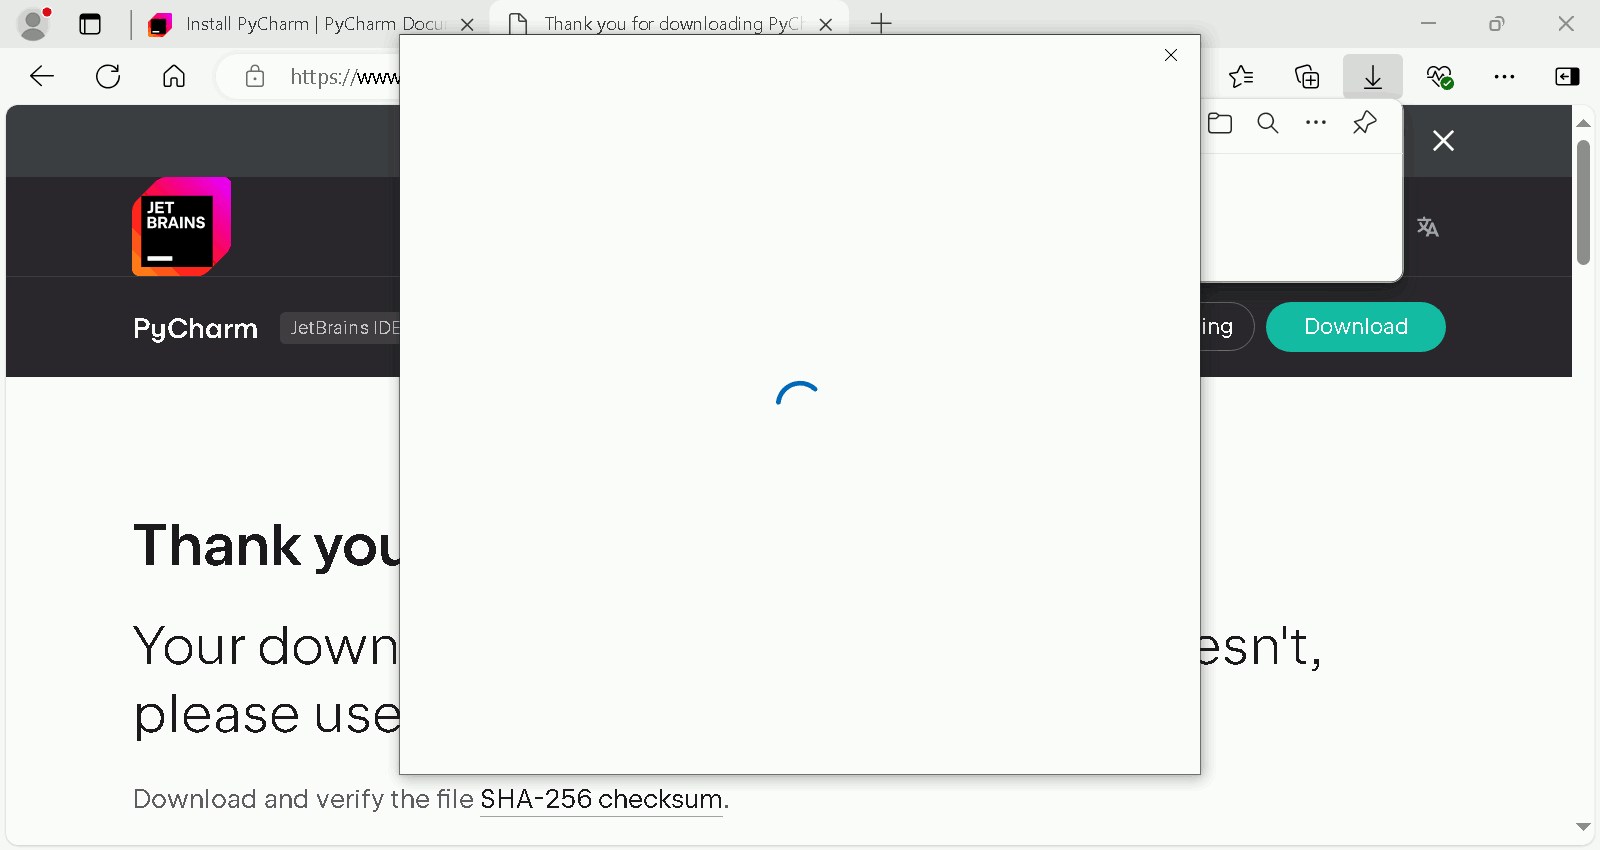
\includegraphics[width=0.7\paperwidth]{graphics/installingPyCharmWindows/installingPyCharmWindows07runInstaller}}}{0.15}{0.29}%
\locate{9}{\tightbox{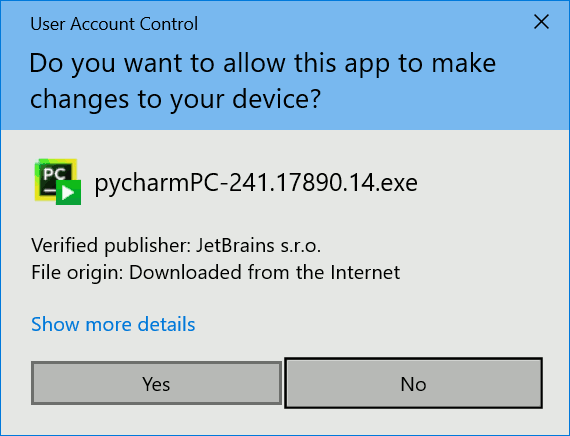
\includegraphics[width=0.5\paperwidth]{graphics/installingPyCharmWindows/installingPyCharmWindows08runInstaller}}}{0.25}{0.27}%
\locate{10}{\tightbox{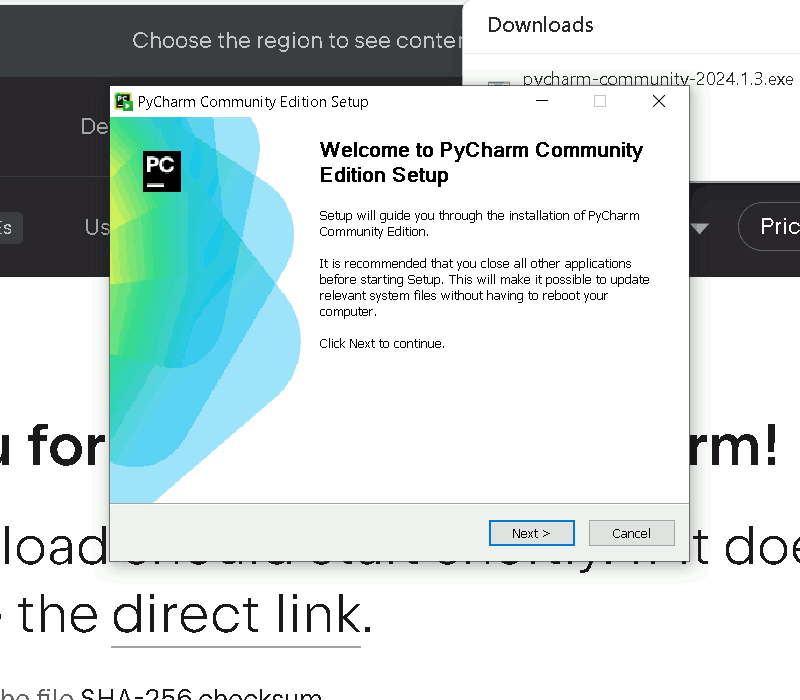
\includegraphics[width=0.5\paperwidth]{graphics/installingPyCharmWindows/installingPyCharmWindows09installation}}}{0.25}{0.26}%
\locate{11}{\tightbox{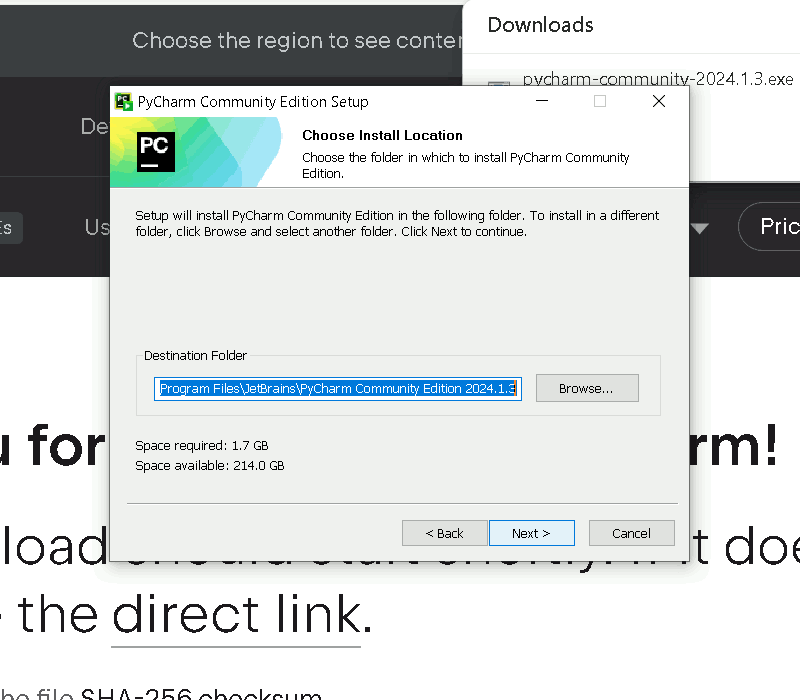
\includegraphics[width=0.5\paperwidth]{graphics/installingPyCharmWindows/installingPyCharmWindows10installation}}}{0.25}{0.25}%
\locate{12}{\tightbox{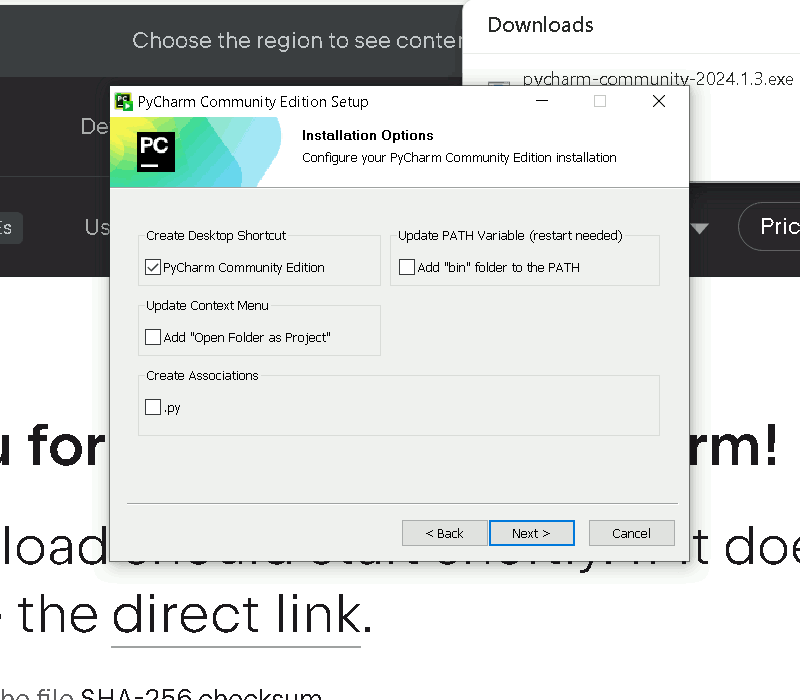
\includegraphics[width=0.5\paperwidth]{graphics/installingPyCharmWindows/installingPyCharmWindows11installation}}}{0.25}{0.25}%
\locate{13}{\tightbox{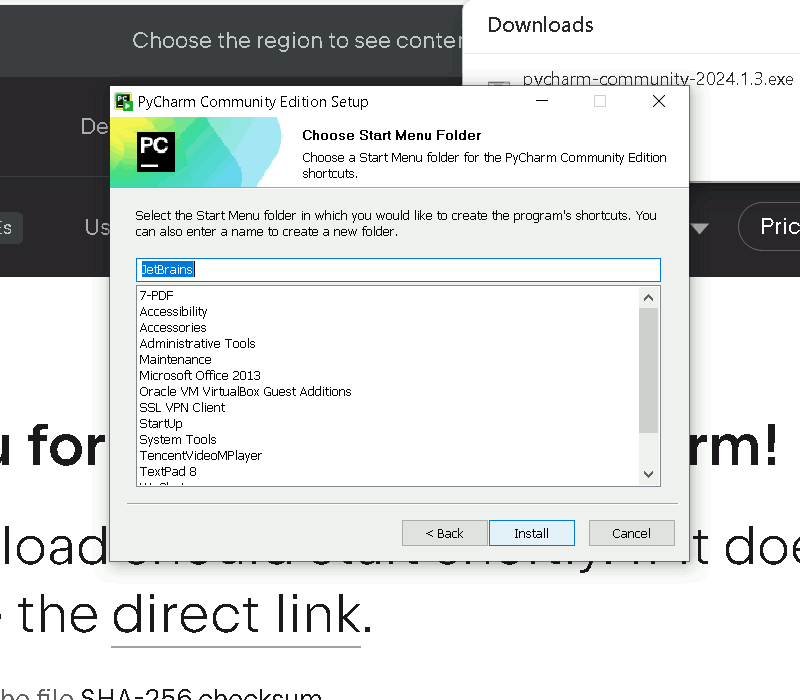
\includegraphics[width=0.5\paperwidth]{graphics/installingPyCharmWindows/installingPyCharmWindows12installation}}}{0.25}{0.25}%
\locate{14}{\tightbox{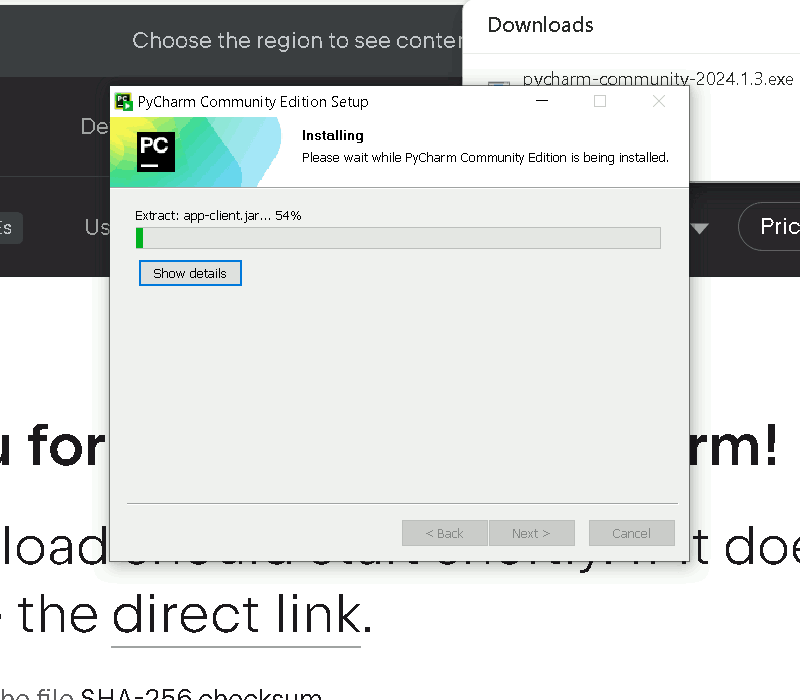
\includegraphics[width=0.5\paperwidth]{graphics/installingPyCharmWindows/installingPyCharmWindows13installation}}}{0.25}{0.25}%
\locate{15}{\tightbox{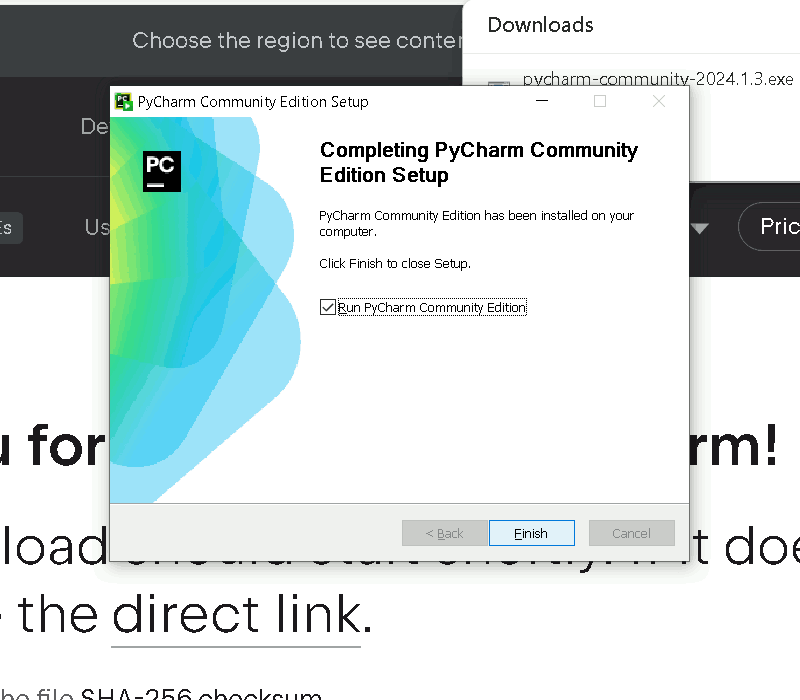
\includegraphics[width=0.5\paperwidth]{graphics/installingPyCharmWindows/installingPyCharmWindows14installation}}}{0.25}{0.27}%
\locate{16}{\tightbox{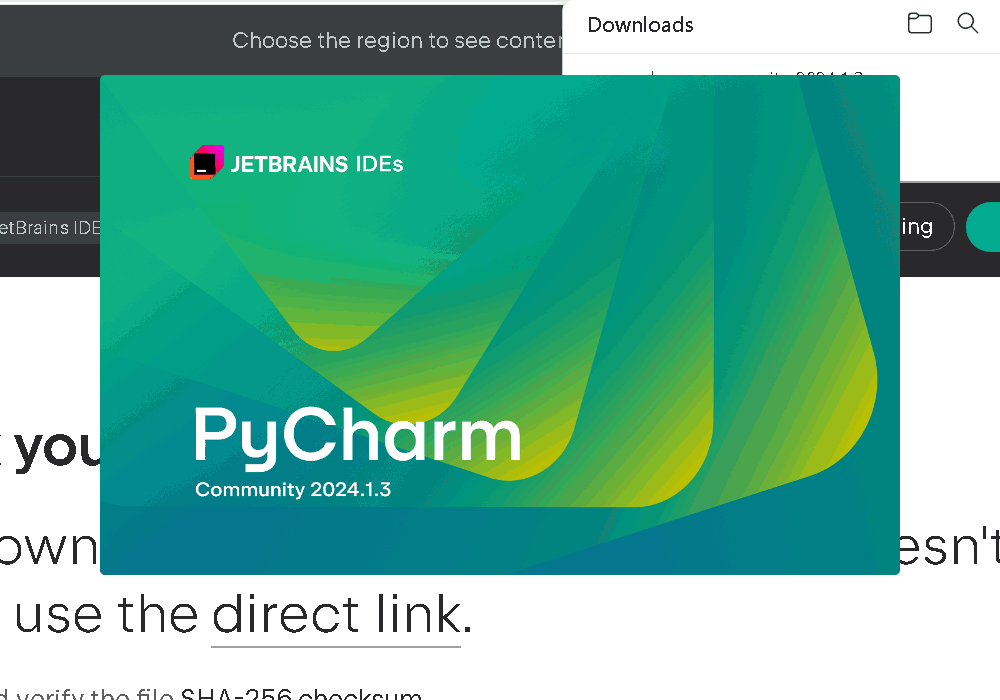
\includegraphics[width=0.5\paperwidth]{graphics/installingPyCharmWindows/installingPyCharmWindows15running}}}{0.25}{0.263}%
\locate{17}{\tightbox{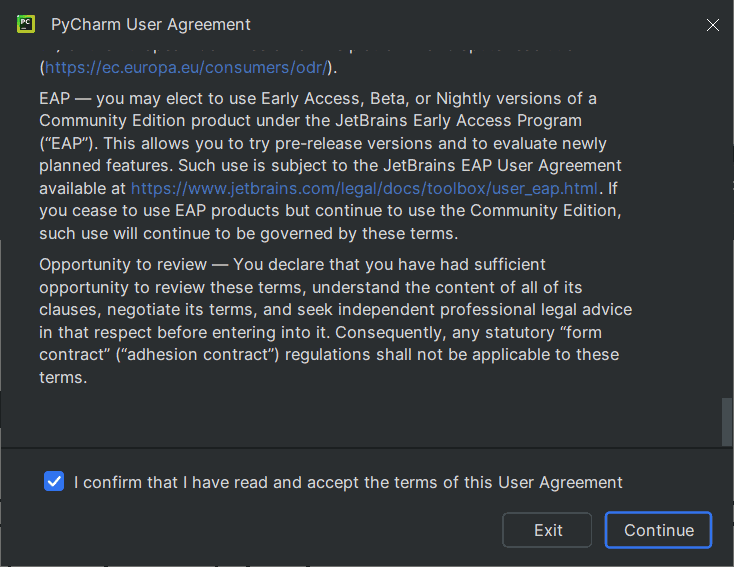
\includegraphics[width=0.5\paperwidth]{graphics/installingPyCharmWindows/installingPyCharmWindows16running}}}{0.25}{0.263}%
\locate{18}{\tightbox{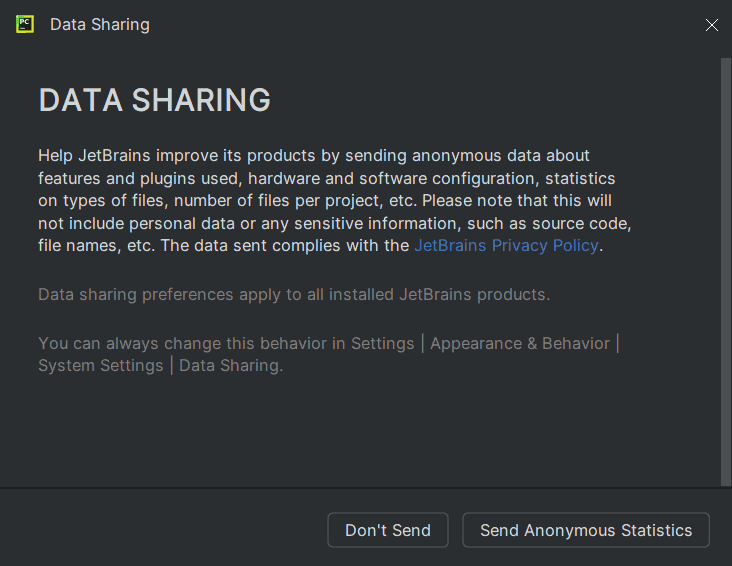
\includegraphics[width=0.5\paperwidth]{graphics/installingPyCharmWindows/installingPyCharmWindows17running}}}{0.25}{0.263}%
\locate{19}{\tightbox{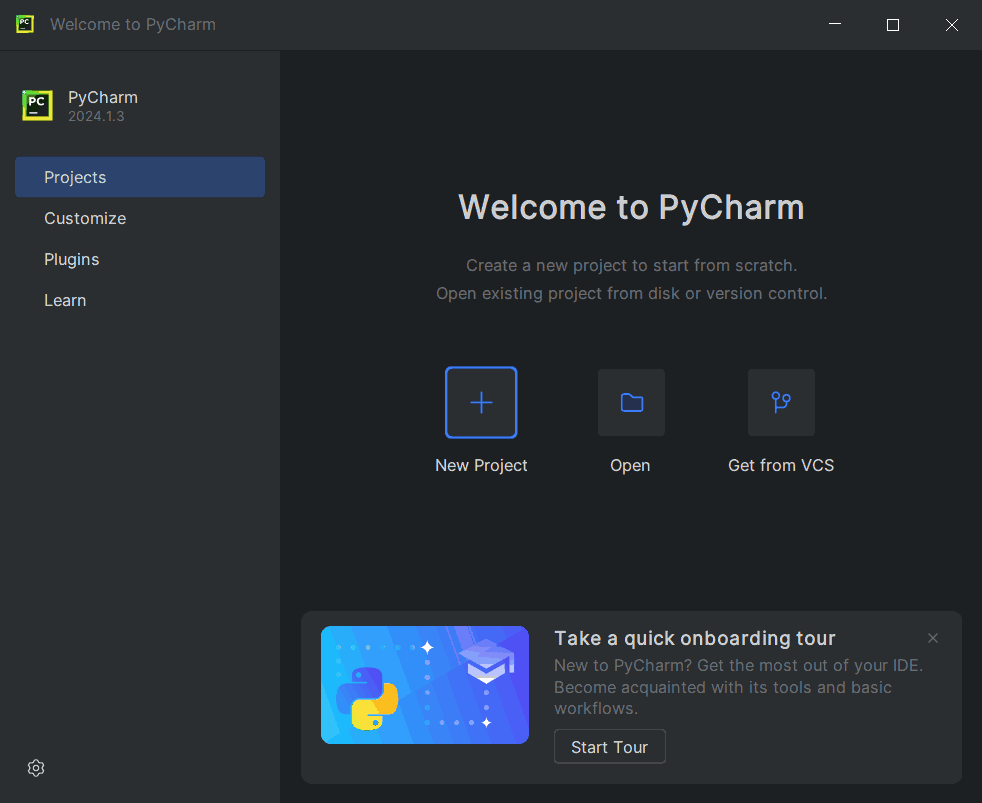
\includegraphics[width=0.5\paperwidth]{graphics/installingPyCharmWindows/installingPyCharmWindows18running}}}{0.25}{0.25}%
%
\end{frame}
%
\section{Our First Program}%
%
\begin{frame}[t]%
\frametitle{Our First Program}%
\begin{itemize}%
\item Let's create a program in \pycharm.%
\end{itemize}%
%
\locate{2}{\tightbox{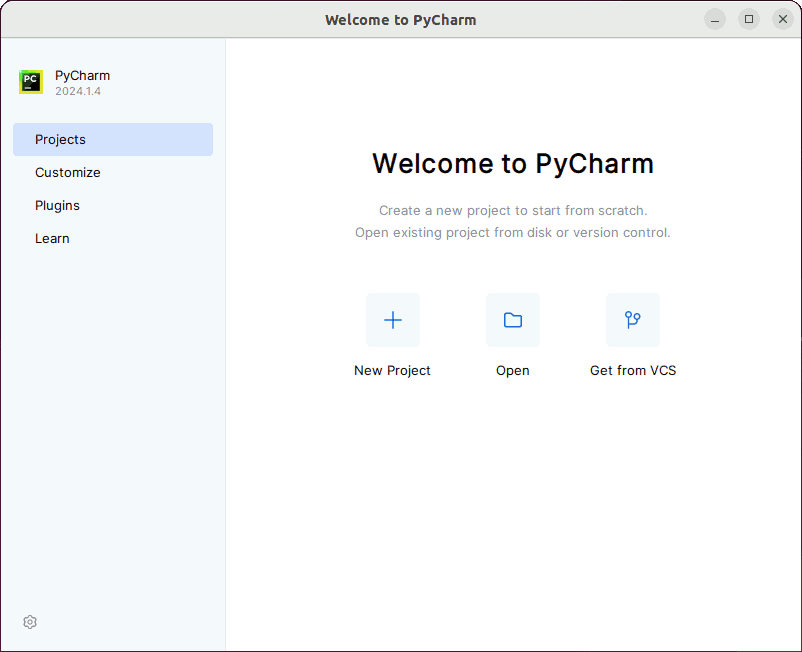
\includegraphics[width=0.5\paperwidth]{graphics/firstProgram/firstProgram01createPyCharmProject}}}{0.25}{0.259}%
\locate{3}{\tightbox{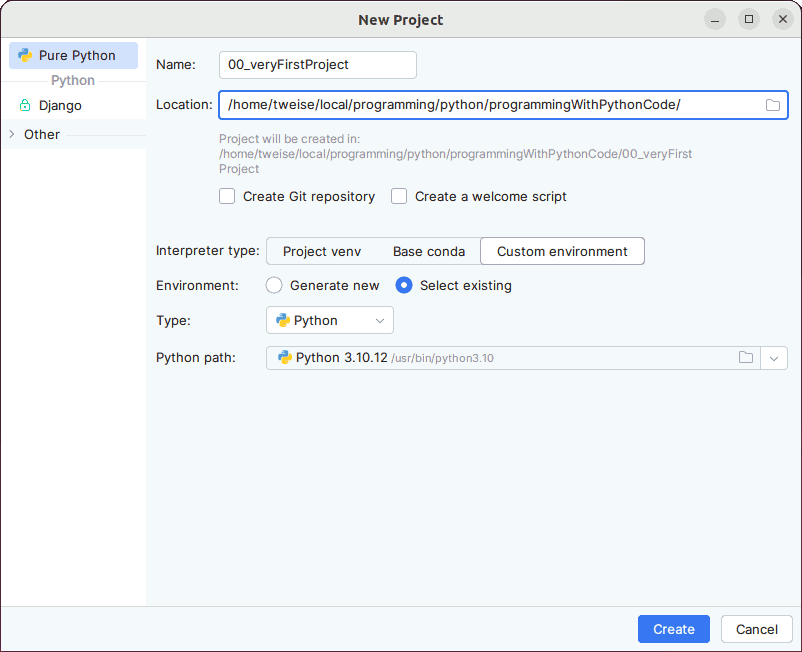
\includegraphics[width=0.5\paperwidth]{graphics/firstProgram/firstProgram02createPyCharmProject}}}{0.25}{0.259}%
\locate{4}{\tightbox{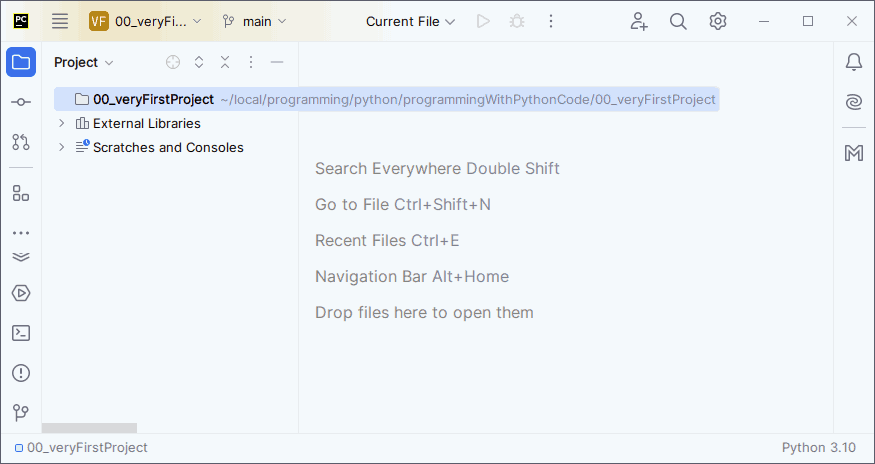
\includegraphics[width=0.7\paperwidth]{graphics/firstProgram/firstProgram03PyCharmProjectCreated}}}{0.15}{0.259}%
\locate{5}{\tightbox{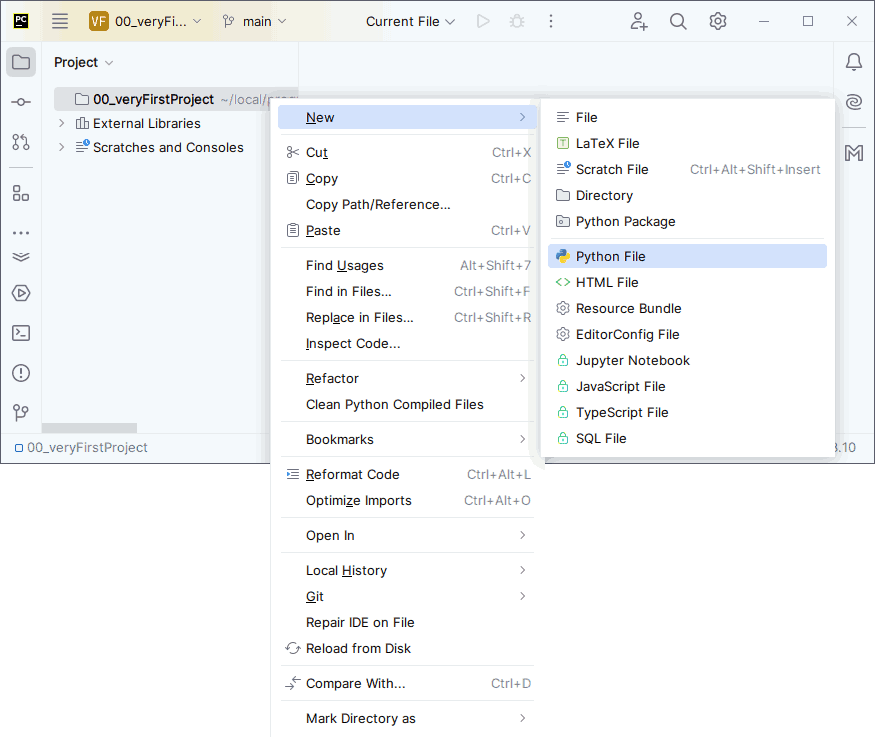
\includegraphics[width=0.5\paperwidth]{graphics/firstProgram/firstProgram04createPythonFile}}}{0.25}{0.259}%
\locate{6}{\tightbox{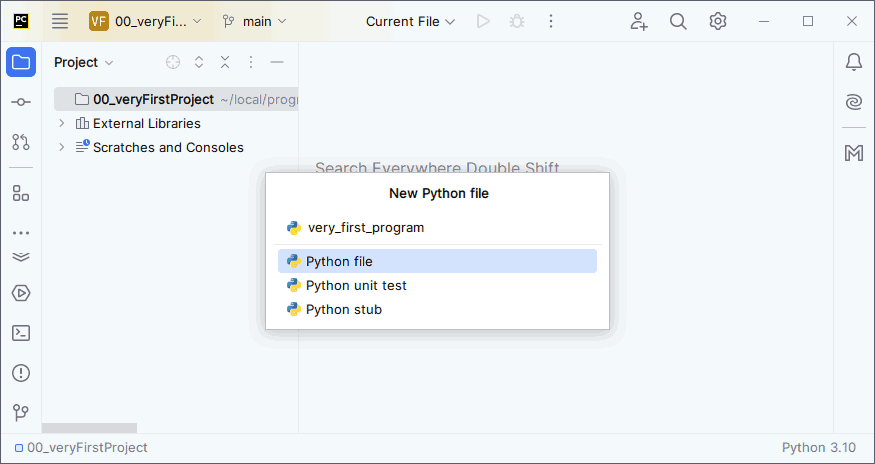
\includegraphics[width=0.7\paperwidth]{graphics/firstProgram/firstProgram05createPythonFile}}}{0.15}{0.259}%
\locate{7}{\tightbox{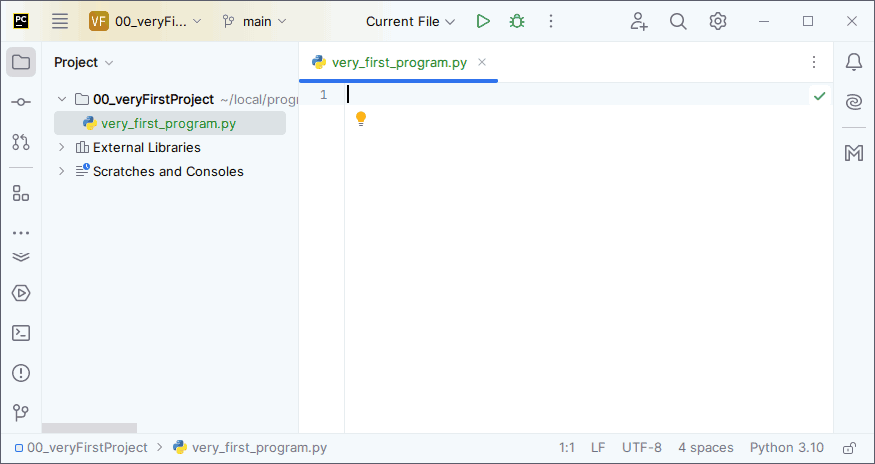
\includegraphics[width=0.7\paperwidth]{graphics/firstProgram/firstProgram06pythonFileCreated}}}{0.15}{0.259}%
\locate{8}{\tightbox{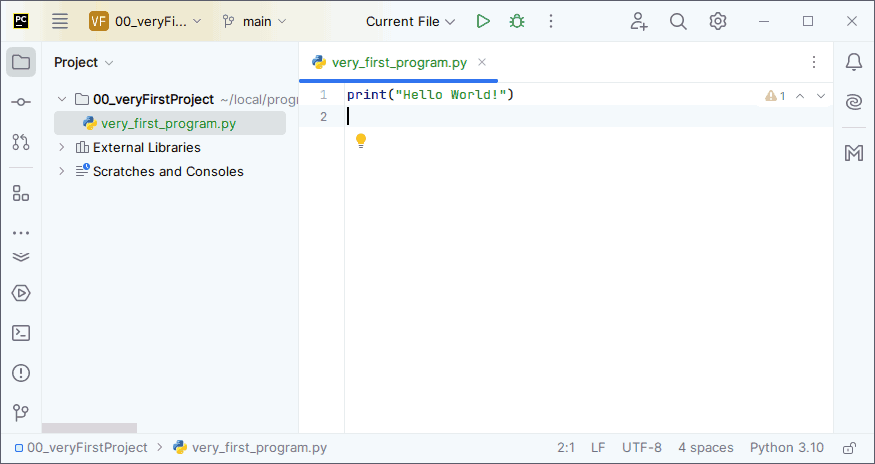
\includegraphics[width=0.7\paperwidth]{graphics/firstProgram/firstProgram07writeHelloWorld}}}{0.15}{0.259}%
\locate{9}{\tightbox{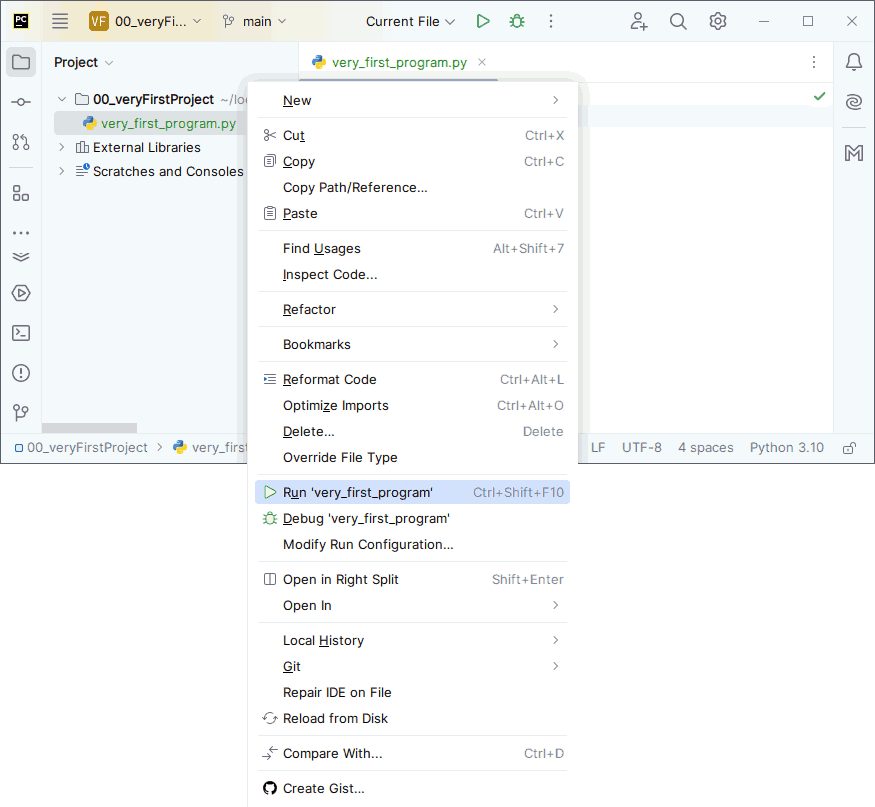
\includegraphics[width=0.5\paperwidth]{graphics/firstProgram/firstProgram08runProgram}}}{0.25}{0.259}%
\locate{10}{\tightbox{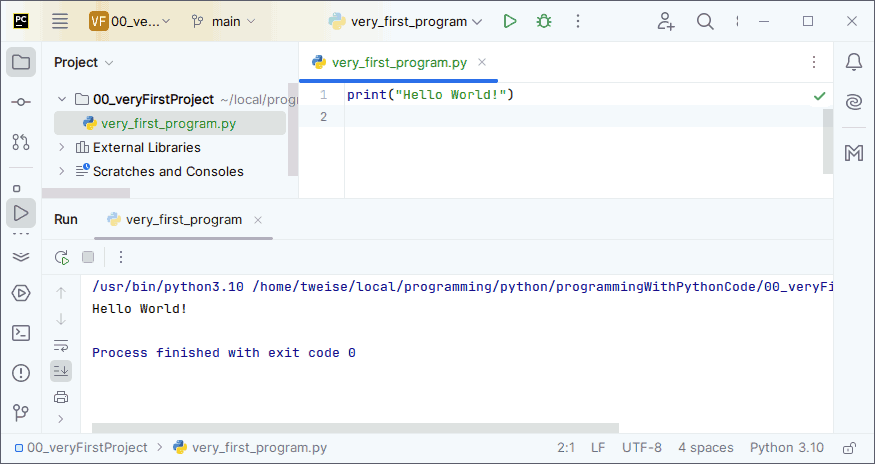
\includegraphics[width=0.7\paperwidth]{graphics/firstProgram/firstProgram09programResult}}}{0.15}{0.259}%
%
%
\end{frame}%
%
%
\section{\python\ in the Terminal}%
%
\begin{frame}[fragile]
\frametitle{Ways to Execute a \python\ Program}%
\begin{itemize}%
%
\item There are at least four ways to run a \python\ program:\uncover<2->{%
\begin{enumerate}%
\item We can enter the program into a \python\ file in the \pycharm\ IDE and then run it from there.%
\item<3-> We can write the program in a normal text editor and store it in a file~\textil{pgogramName.py}.\uncover<4->{ %
Then we can open a terminal, enter the directory, and type~\bashil{python3 programName.py} and hit~\keys{\enter}.\uncover<5->{ %
This executes the program in the terminal.}}%
%
\item<6-> We can open the \python\ interpreter console in \pycharm\ and enter and execute our code line-by-line.%
%
\item<7-> We can use the \python\ console inside a terminal.\uncover<8->{ %
We can then enter separate \python\ instructions and run them there.}%
\end{enumerate}}%
%
\item<8-> We already did option~\enumerateItem{1}, now let's try the others.%
%
\end{itemize}%
\end{frame}
%
\begin{frame}[fragile,t]
\frametitle{Execute a python Program in the Terminal}
\begin{itemize}%
\item Open a terminal by pressing \ubuntuTerminal\ under \ubuntu\ \linux; under \microsoftWindows\ \windowsTerminal.%
\end{itemize}%
%
\locate{2}{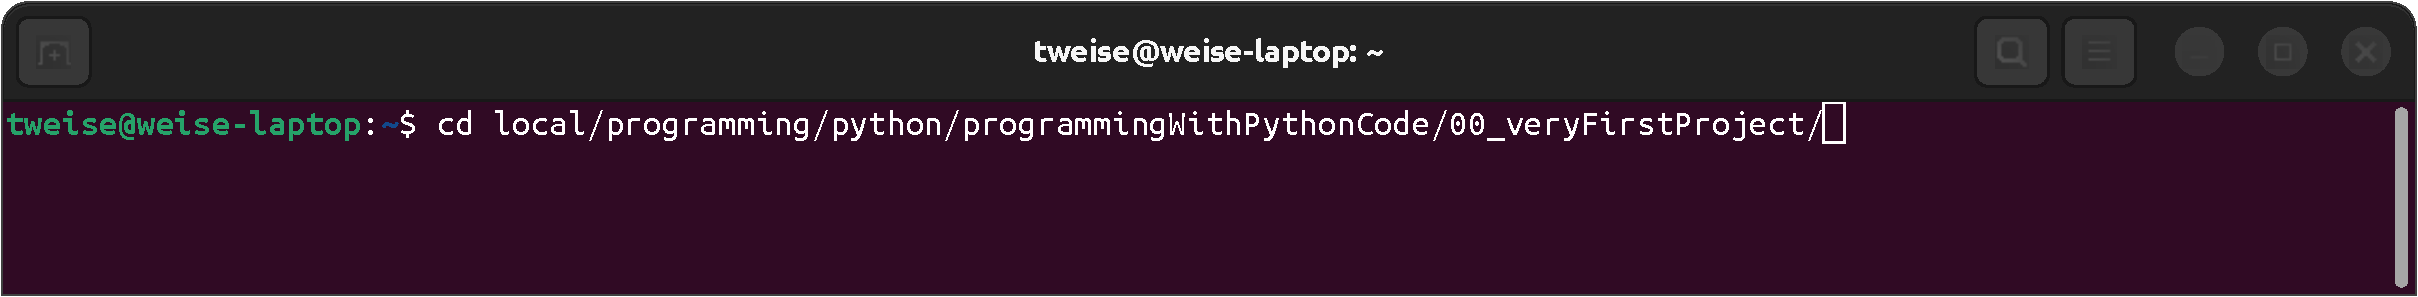
\includegraphics[width=0.8\paperwidth]{graphics/pythonInTheTerminal/terminalPython1cd}}{0.1}{0.4}%
\locate{3}{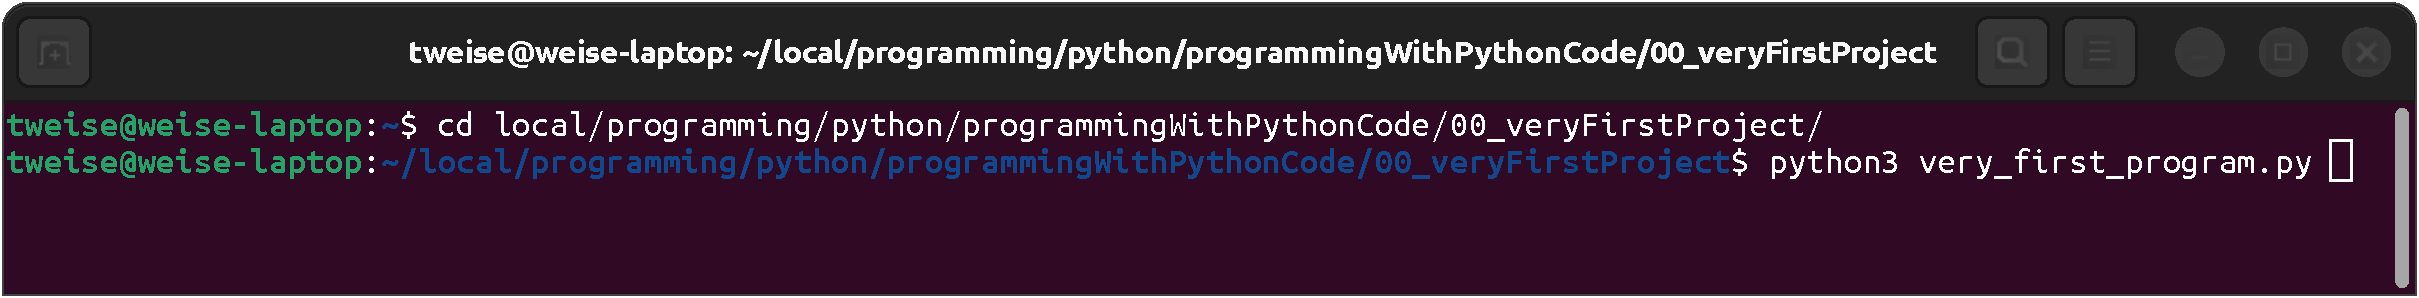
\includegraphics[width=0.8\paperwidth]{graphics/pythonInTheTerminal/terminalPython2python}}{0.1}{0.4}%
\locate{4}{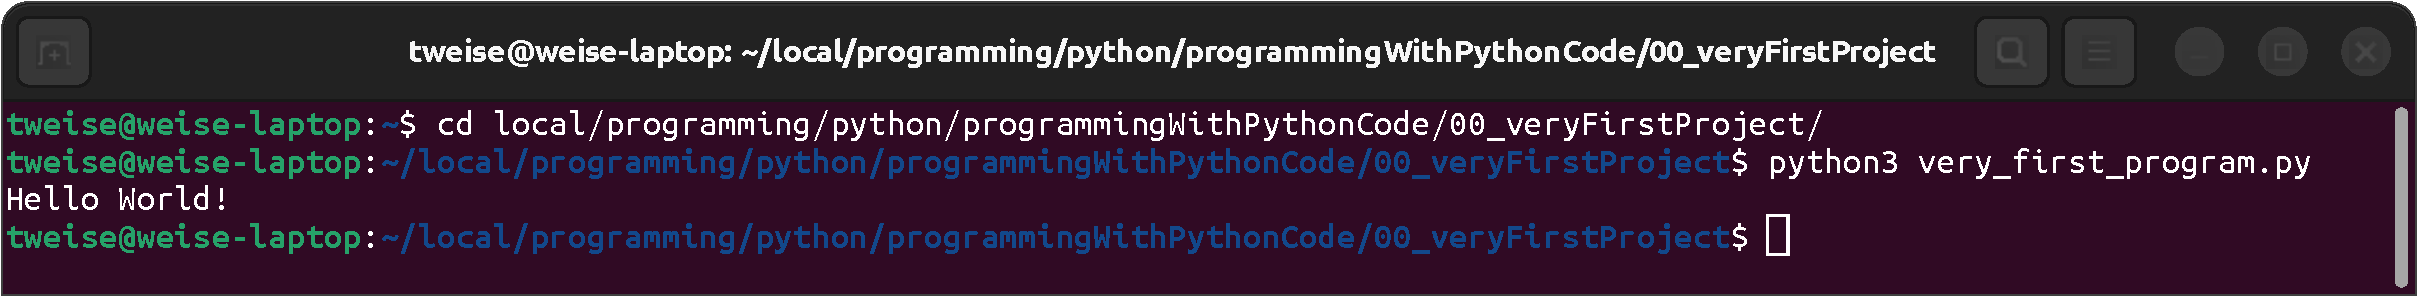
\includegraphics[width=0.8\paperwidth]{graphics/pythonInTheTerminal/terminalPython3result}}{0.1}{0.4}%
%
\gitPythonAndOutput{6}{\programmingWithPythonCodeRepo}{veryFirstProject}{very_first_program.py}{--args format}{0.05}{0.45}{0.9}{0.8}%
%
\end{frame}
%
\begin{frame}[t]%
\frametitle{Entering Commands in the \python\ Console inside \pycharm}%
%
\begin{itemize}%
\item We can also directly enter programs into the \pycharm\ \python\ console (press \menu{\pycharmConsole}) and execute them step-by-step.%
\item<2-> This does not make sense if we want to reuse our programs later.%
\end{itemize}%
%
\locate{3}{\tightbox{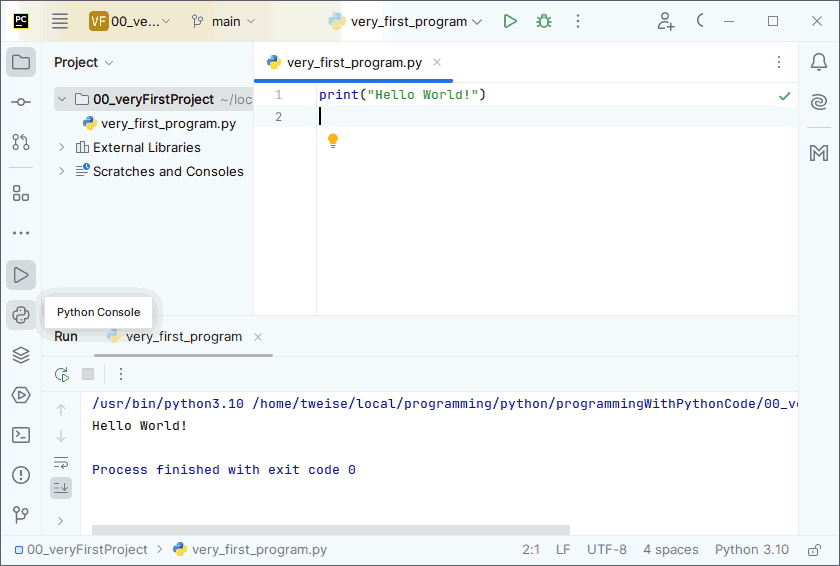
\includegraphics[width=0.5\paperwidth]{graphics/pythonInTheTerminal/pycharmConsole1consoleButton}}}{0.25}{0.35}%
\locate{4}{\tightbox{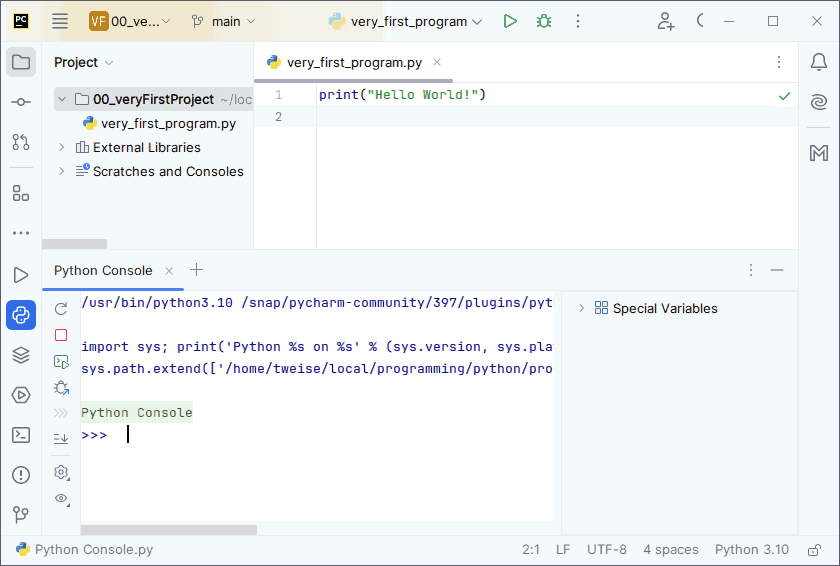
\includegraphics[width=0.5\paperwidth]{graphics/pythonInTheTerminal/pycharmConsole2consoleOpen}}}{0.25}{0.35}%
\locate{5}{\tightbox{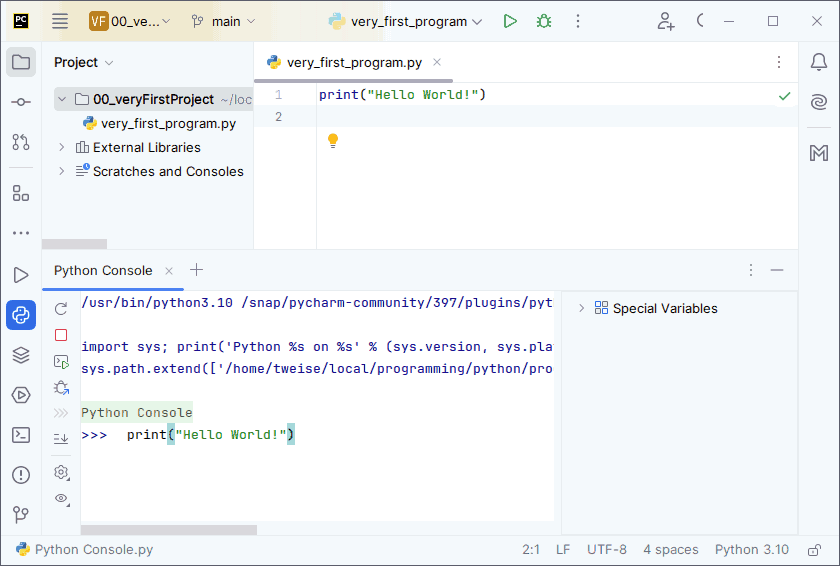
\includegraphics[width=0.5\paperwidth]{graphics/pythonInTheTerminal/pycharmConsole3writingCode}}}{0.25}{0.35}%
\locate{6}{\tightbox{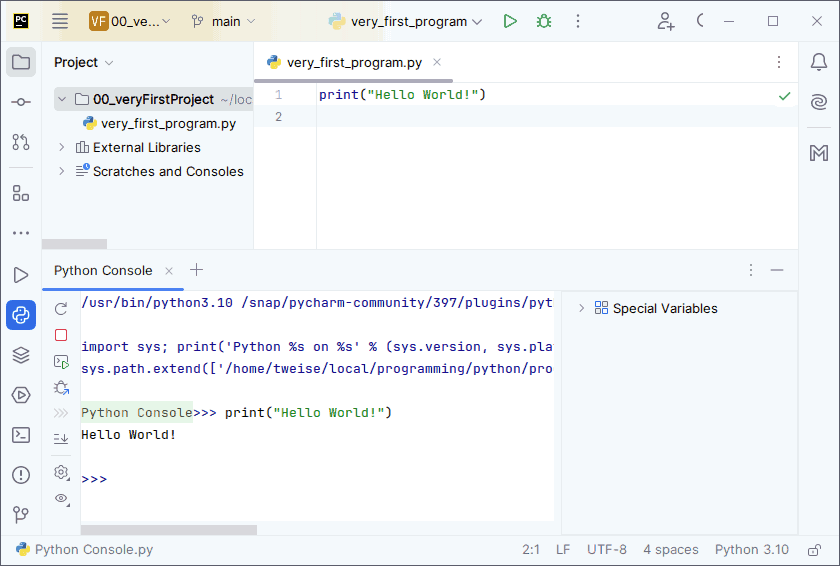
\includegraphics[width=0.5\paperwidth]{graphics/pythonInTheTerminal/pycharmConsole4codeOutput}}}{0.25}{0.35}%
%
\end{frame}%
%
\begin{frame}[t]%
\frametitle{Entering Commands in the \python\ Console in a Terminal}%
\begin{itemize}%
\item {\dots}or we can open a \python\ console in a terminal.%
\end{itemize}%
%
\locate{2}{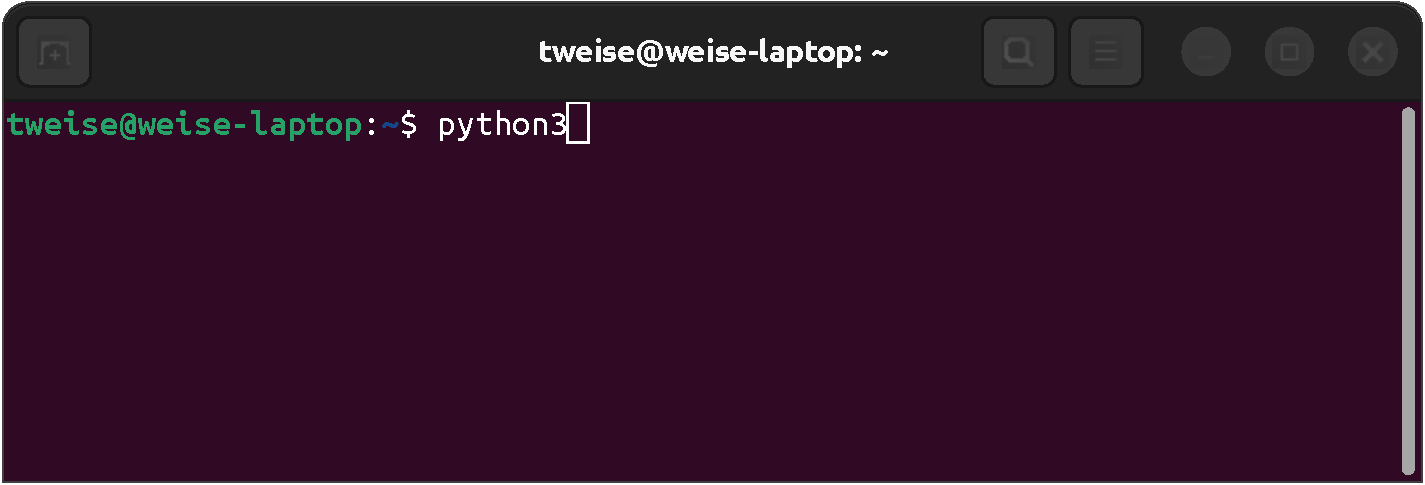
\includegraphics[width=0.7\paperwidth]{graphics/pythonInTheTerminal/terminalConsole1python}}{0.15}{0.35}%
\locate{3}{\includegraphics[width=0.7\paperwidth]{graphics/pythonInTheTerminal/terminalConsole2pythonRunning}}{0.15}{0.35}%
\locate{4}{\includegraphics[width=0.7\paperwidth]{graphics/pythonInTheTerminal/terminalConsole3writingCode}}{0.15}{0.35}%
\locate{5}{\includegraphics[width=0.7\paperwidth]{graphics/pythonInTheTerminal/terminalConsole5exit}}{0.15}{0.35}%
\locate{6}{\includegraphics[width=0.7\paperwidth]{graphics/pythonInTheTerminal/terminalConsole6left}}{0.15}{0.35}%
\end{frame}%
%
\begin{frame}[fragile]
\frametitle{Ways to Execute a \python\ Program}%
\begin{itemize}%
%
\item There are at least four ways to run a \python\ program:%
\begin{enumerate}%
\item We can enter the program into a \python\ file in the \pycharm\ IDE and then run it from there.%
\item We can write the program in a normal text editor and store it in a file~\textil{pgogramName.py}. %
Then we can open a terminal, enter the directory, and type~\bashil{python3 programName.py} and hit~\keys{\enter}. %
This executes the program in the terminal.%
%
\item We can open the \python\ interpreter console in \pycharm\ and enter and execute our code line-by-line.%
%
\item We can use the \python\ console inside a terminal. %
We can then enter separate \python\ instructions and run them there.%
\end{enumerate}%
%
\bestPractice{runningProgram}{The only proper way to run a \python\ application in a productive scenario is in the terminal.}%
\end{itemize}%
\end{frame}
%
%
\section{Obtaining the Examples}%
%
\begin{frame}[t]%
\frametitle{Downloading the Examples}%
\begin{itemize}%
\item This course is practice-centered, so it comes with lots of examples.
\item<2-> You can download them from \expandafter\url{\programmingWithPythonCodeRepo/archive/refs/heads/main.zip}.%
\end{itemize}%
%
\locate{3}{\tightbox{\includegraphics[width=0.45\paperwidth]{graphics/examples/downloadExamples}}}{0.275}{0.35}%
\end{frame}%
%
\begin{frame}[t]%
\frametitle{Clone Repository in \pycharm}%
\begin{itemize}%
\item You can also clone the repository \expandafter\url{\programmingWithPythonCodeRepo} in \pycharm.%
\end{itemize}%
%
\locate{2}{\tightbox{\includegraphics[width=0.45\paperwidth]{graphics/examples/clone01welcomeToPycharm}}}{0.275}{0.263}%
\locate{3}{\tightbox{\includegraphics[width=0.45\paperwidth]{graphics/examples/clone02selectRepoAndDestination}}}{0.275}{0.263}%
\locate{4}{\tightbox{\includegraphics[width=0.45\paperwidth]{graphics/examples/clone03cloning}}}{0.275}{0.263}%
\locate{5}{\tightbox{\includegraphics[width=0.65\paperwidth]{graphics/examples/clone04trustProject}}}{0.175}{0.263}%
\locate{6}{\tightbox{\includegraphics[width=0.65\paperwidth]{graphics/examples/clone05finished}}}{0.175}{0.263}%
%
\end{frame}%
%
\section{Summary}%
%
\begin{frame}\frametitle{Summary}%
\begin{itemize}%
\item The optimization algorithms we consider in this lecture are \alert<1>{randomized}.%
\end{itemize}%
\end{frame}%
%
\endPresentation%
\end{document}%%
\endinput%
%
